\subsection{Test Scenarios}
\import{sections/design/}{testscenarios.tex}
\import{sections/design/}{testtables.tex}
\pagebreak
\subsection{Compile Flags}
While there was not enough time remaining to implement any for of automated program testing mode into the program, I decided to make use of compile time flags to make running certain tests easier to run or simply possible to run. Such as selecting the particular test scenario, changing initial state or modifying the operation of the system. These are achived through the use of constant declare conditional statements for the compiler preprocessor in code.

\paragraph{}
These compile flags can be used by compiling the program with the makefile, calling with:
\begin{lstlisting}[language=bash]
  make -j12 CS="-DDEFAULT -DSIMITRS=10"
\end{lstlisting}
\paragraph{}
The \textit{-j12} argument enables parallel compilation, which compiles separate source files at the same time in order to decrease the total time taken to compile the program, in this case it allows for 12 concurrent jobs, this is excessive for the number of files compiled in this program, but it should be set to the number of available concurrent threads on the system the application is being compiled on.

\paragraph{}
Because of the way that the makefile has been written, files that have had no change to their source code will not recompile if the object files still exist, this speeds up the compile time by only compiling the files that need to be recompiled. \\
Because of this however, \textit{make clean} must be run first in order to delete the current executable and all existing object code files before the changes to the compile flags take effect.

\paragraph{}
The following is a list of all of the currently implemented flags that can be defined at compile time to modify the function of the program for testing.\\
\begin{itemize}
\footnotesize
\item \textbf{DEFAULT} - Sets the default start-up scenario.
\item \textbf{TS1} - 12 - Sets the start-up scenario to one of the predefined test scenarios.
\item \textbf{SIMITRS} - Sets a limit to the number of iterations that the simulation will run for. (This does require the program to force close as the simulation thread exits early.)
\item \textbf{SIPF} - Causes an 'i' to be printed to the cout stream on every iteration, not just rendered frames. Newline is printed when frame is sent to shared.
\item \textbf{SCI} - Prints the current iteration since program launch when it is paused.
\item \textbf{PRINTV} - Prints the XY velocity of all bodies every iteration.
\item \textbf{PRINTV} - Prints the XY position of all bodies every iteration.
\item \textbf{PRINTAC} - Prints A and B being calculated in the acceleration calculation. (Relationships being calculated)
\item \textbf{PRINTFORCE} - Prints the result of the force calculated for each relationship. 
\item \textbf{PRINTMXY} - Print current mouse XY coordinates. (Window coordinates)
\item \textbf{PRINTMACT} - Print current mouse XY coordinates on mouse click. (World coordinates)
\item \textbf{EXITNOTE} - Prints notifications for simulation thread exit and main thread exit.
\item \textbf{NOSYNC} - Removes thread synchronisation, allows for the simulation to run much faster than simulation, can cause issues.
\item \textbf{C\_UGC} - Custom gravitational constant.
\item \textbf{C\_IDT} - Custom iteration delta time.
\item \textbf{C\_PAUSED} - Custom paused switch.
\item \textbf{C\_COLLIDE} - Custom collision switch.
\item \textbf{TS4BODIES} - Declares the numbers that will be generated by the TS4 superstructure.
\end{itemize}

\subsubsection{System Tests}
\begin{itemize}
\footnotesize
\item \textbf{SYS1} - DEFAULT
\item \textbf{SYS2} - DEFAULT
\item \textbf{SYS3} - 
\item \textbf{SYS4} - DEFAULT
\item \textbf{SYS5} - EXITNOTE
\item \textbf{SYS6} - DEFAULT
\end{itemize}

\subsubsection{Interface Tests}
\begin{itemize}
\footnotesize
\item \textbf{GUI1} - TS7, C\_UGC=0, PRINTMACT, PRINTMXY
\item \textbf{GUI2} - TS7, C\_UGC=0, PRINTMACT
\item \textbf{GUI3} - TS7, C\_UGC=0, PRINTMACT
\item \textbf{GUI4} - TS7, C\_UGC=0, PRINTMACT
\item \textbf{GUI5} - TS7, C\_UGC=0, PRINTMACT
\item \textbf{GUI6} - 
\item \textbf{GUI7} - PRINTMACT
\item \textbf{GUI8} - 
\item \textbf{GUI9} - 
\item \textbf{GUI10} - DEFAULT
\item \textbf{GUI11} - 
\item \textbf{GUI12} - 
\item \textbf{GUI13} - 
\item \textbf{GUI14} - DEFAULT
\item \textbf{GUI15} - DEFAULT
\item \textbf{GUI16} - TS8, SIPF
\item \textbf{GUI17} - TS7, C\_UGC=0
\end{itemize}

\subsubsection{Simulation Tests}
\begin{itemize}
\footnotesize
\item \textbf{SIM1} - TS1, SIMITRS=10
\item \textbf{SIM2} - TS2, SIMITRS=1
\item \textbf{SIM3} - TS2, SIMITRS=1
\item \textbf{SIM4} - TS2, SIMITRS=6283
\item \textbf{SIM5} - TS2, SIMITRS=6283
\item \textbf{SIM6} - TS3, C\_UGC=0, C\_PAUSED=1
\item \textbf{SIM7} - TS3, C\_UGC=0, C\_PAUSED=1
\item \textbf{SIM8} - TS3, C\_UGC=0, C\_PAUSED=1
\item \textbf{SIM9} - TS3, C\_UGC=0, C\_PAUSED=1
\item \textbf{SIM10} - TS4, TS4BODIES=Variable, C\_COLLIDE=0, C\_PAUSED=1, NOSYNC, SCI
\item \textbf{SIM11} - TS5, C\_PAUSED=1
\item \textbf{SIM12} - TS6, C\_PAUSED=1
\item \textbf{SIM13} - TS9, SIMITRS=8, C\_IDT=2, PRINTV, PRINTP
\item \textbf{SIM14} - TS8, C\_PAUSED=1
\item \textbf{SIM15} - TS11, C\_IDT=0.01, C\_PAUSED=1
\item \textbf{SIM16} - TS11, C\_IDT=0.01, C\_PAUSED=1
\item \textbf{SIM17} - 
\item \textbf{SIM18} - TS11, SIMITRS=1, PRINTAC
\item \textbf{SIM19} - TS12, SIMITRS=1, PRINTAC, PRINTFORCE, C\_UGC=10
\end{itemize}

\pagebreak
\subsection{Test Results}
\subsubsection{System Tests}
\begin{itemize}
\footnotesize
\item \textbf{SYS1} - {\color{Red}Fail}, \textbf{see notes}, {\color{Green}Pass}
\item \textbf{SYS2} - {\color{Green}Pass}
\item \textbf{SYS3} - {\color{Green}Pass}
\item \textbf{SYS4} - {\color{Green}Pass}
\item \textbf{SYS5} - {\color{Green}Pass}
\item \textbf{SYS6} - {\color{Green}Pass}
\end{itemize}

\subsubsection{Interface Tests}
\begin{itemize}
\footnotesize
\item \textbf{GUI1} - {\color{Green}Pass}
\item \textbf{GUI2} - {\color{Green}Pass}
\item \textbf{GUI3} - {\color{Green}Pass}
\item \textbf{GUI4} - {\color{Green}Pass}
\item \textbf{GUI5} - {\color{Green}Pass}
\item \textbf{GUI6} - {\color{Green}Pass}
\item \textbf{GUI7} - {\color{Green}Pass}
\item \textbf{GUI8} - {\color{Green}Pass}
\item \textbf{GUI9} - {\color{Green}Pass}
\item \textbf{GUI10} - {\color{Green}Pass}
\item \textbf{GUI11} - {\color{Green}Pass}
\item \textbf{GUI12} - {\color{Green}Pass}
\item \textbf{GUI13} - {\color{Green}Pass}
\item \textbf{GUI14} - $0$ {\color{Green}Pass}, $10$ {\color{Green}Pass}, $\num{1E3}$ {\color{Green}Pass}, $152$ {\color{Green}Pass}
\item \textbf{GUI15} - $\num{1E18}$ {\color{Green}Pass}, $ABC$ {\color{Green}Pass}, $\num{-1E17}$ {\color{Green}Pass}, $asdfseaq$ {\color{Green}Pass}
\item \textbf{GUI16} - $1$ {\color{Green}Pass}, $2$ {\color{Green}Pass}, $5$ {\color{Green}Pass}, $32$ {\color{Green}Pass},
\item \textbf{GUI17} - {\color{Green}Pass}
\end{itemize}

\subsubsection{Simulation Tests}
\begin{itemize}
\footnotesize
\item \textbf{SIM1} - {\color{Green}Pass}
\item \textbf{SIM2} - {\color{Green}Pass}
\item \textbf{SIM3} - {\color{Green}Pass}
\item \textbf{SIM4} - {\color{Green}Pass}
\item \textbf{SIM5} - {\color{Green}Pass}
\item \textbf{SIM6} - {\color{Green}Pass}
\item \textbf{SIM7} - Mass $[10,1]$ {\color{Green}Pass}, $[20,100]$ {\color{Green}Pass}, $[1000,1000]$ {\color{Green}Pass},
\item \textbf{SIM8} - Velocity $[-1,1]$ {\color{Green}Pass}, $[2,1]$ {\color{Green}Pass}, $[-150,150]$ {\color{Red}Fail}, \textbf{see notes},
\item \textbf{SIM9} - Radius $[10,1]$ {\color{Green}Pass}, $[20,100]$ {\color{Green}Pass}, $[1000,1000]$ {\color{Green}Pass},
\item \textbf{SIM10} - $10, 20, 40, 80, 100, 200, 400, 800, 1000, 2000, 4000, 10000$ {\color{Green}Pass}, \textbf{see notes}
\item \textbf{SIM11} - {\color{Green}Pass}
\item \textbf{SIM12} - {\color{Green}Pass}
\item \textbf{SIM13} - {\color{Green}Pass}
\item \textbf{SIM14} - {\color{Green}Pass}
\item \textbf{SIM15} - {\color{Green}Pass}
\item \textbf{SIM16} - {\color{Green}Pass}
\item \textbf{SIM17} - {\color{Green}Pass}
\item \textbf{SIM18} - {\color{Green}Pass}
\item \textbf{SIM19} - {\color{Green}Pass}
\end{itemize}

\subsection{Test Notes}
\subsubsection{SYS1}
Test SYS1 initially failed due to an incompatibility with the test program Valgrind and C++ call \textit{random\_device}, which is intended to get a random seed every time the application starts instead of using the current time as a seed.
\paragraph{}
For an unknown reason, this code causes Valgrind to crash on the desktop PC that was running the test, but not on a secondary PC. To get around this, the \textit{random\_device} code was removed during all of the tests that involved the use of Valgrind and a static seed was used.
\subsubsection{SIM8}
SIM8 was successful on all but the last test, where the two bodies are moving towards each other with a velocity of 150 each, due to this speed, the bodies end up not registering a collision and continue on past each other.
\paragraph{}
This is due to a number of factors, but it is a context dependant issue and not something that can be easily rectified in the current algorithm.
\paragraph{}
The cause of this issue is related to the velocity, however it is also dependant on the radius of the objects and the current delta time of the simulation, effectively the velocity of the bodies is so great that they end up moving past each other in the space of a single time step, thus their bounds never collide and a collision does not register and calculate.
\paragraph{}
The solution to this is to either increase the radius of the objects or decrease the timestep, in terms of algorithm, the only solution on that end would be to reduce the timestep when bodies are detected as being close together and going too fast to catch the collision. This would require extensive profiling to ensure that this would work efficiently, it may also cause some instability in terms of the simulation due to the way that leapfrog integration works.
\subsubsection{SIM10}
SIM10 was a quantitative benchmark to examine the performance of the simulation and observe the increase in computational time compared to the number of bodies.
\paragraph{}
At each test point, the simulation was allowed to run for 20s and the number of iterations carried out was recorded, 6 repeats were carried out for each test point to provide a better average.\\

\begin{table}[h]
\footnotesize
\centering
\caption{Simulation Benchmark - Iterations in 20s}
\def\arraystretch{1.5}
\begin{tabular}{|c|c|c|c|c|c|c|c|} \hline
Bodies & $i_1$ & $i_2$ & $i_3$ & $i_4$ & $i_5$ & $i_6$ & $i_{mean}$\\ \hline
    11 & 13300000 & 13600000 & 13400000 & 13400000 & 13600000 & 13000000 & \textbf{13433333} \\ \hline
    21 &	4890000	&  4830000 &	4870000 &  4800000 &	4880000 &	 4790000 &	\textbf{4843333} \\ \hline
    41 &	1500000	&  1490000 &	1500000 &  1500000 &	1490000 &  1500000 &  \textbf{1496667} \\ \hline
    81 &   426000 &   419000 &   419000 &   417000 &   423000 &   417000 &   \textbf{420167} \\ \hline
   101 &   271000 &   278000 &   278000 &   272000 &   275000 &   274000 &   \textbf{274667} \\ \hline
   201 &    72100 &    71800 &    72000 &    71800 &    71800 &    72100 &    \textbf{71933} \\ \hline
   401 &    18400 &    18300 &    18500	&    18700 &    18500 &    18400 &    \textbf{18467} \\ \hline
   801 &     4650	&     4690 &     4640 &   	4650 &     4650 &    	4690 &     \textbf{4662} \\ \hline
  1001 &     3021	&     3000 &     2980 &   	2970 &     3030 &   	3000 &     \textbf{3000} \\ \hline
  2001 &      756	&      751 &	    752 &	     750 &	    748 &	     743 &      \textbf{750} \\ \hline
  4001 &      190 &	     188 &	    187 &      188 &	    187 &    	 186 &      \textbf{188} \\ \hline
  8001 &       47 &	      46 &       47 &	      46 &       46 &	      47 &       \textbf{47} \\ \hline
 10001 &       30 &	      29 &       29 &	      30 &       30 &	      29 &       \textbf{30} \\ \hline
\end{tabular}
\end{table}

\pagebreak

\begin{wraptable}{l}{5.5cm}
\footnotesize
\centering
\caption{Per Second}
\def\arraystretch{1.5}
\begin{tabular}{|c|c|c|} \hline
Bodies & $i_{1s}$ & $T_i$\\ \hline
    11 & 670000   & \SI{  1}{\micro\second}  \\ \hline
    21 & 240000   & \SI{  4}{\micro\second}  \\ \hline
    41 &  75000   & \SI{ 13}{\micro\second}  \\ \hline
    81 &  21000   & \SI{ 47}{\micro\second}  \\ \hline
   101 &  14000   & \SI{ 71}{\micro\second}  \\ \hline
   201 &   3600   & \SI{280}{\micro\second}  \\ \hline
   401 &    920   & \SI{  1}{\milli\second}  \\ \hline
   801 &    230   & \SI{  4}{\milli\second}  \\ \hline
  1001 &    150   & \SI{  7}{\milli\second}  \\ \hline
  2001 &     38   & \SI{ 27}{\milli\second}  \\ \hline
  4001 &      9.4 & \SI{110}{\milli\second}  \\ \hline
  8001 &      2.3 & \SI{440}{\milli\second}  \\ \hline
 10001 &      1.5 & \SI{670}{\milli\second}  \\ \hline
\end{tabular}
\vspace{-40pt}
\end{wraptable}

\paragraph{}
By processing this data and getting the reciprocal of the number of iterations in a second, the total time per iteration can be found, the figures in this table have been rounded for clarity.

\paragraph{}
With this data graphs can be created to better represent the performance of the simulation and allow for approximation of performance at other body counts, based on said graphs the simulation will remain at 60 frames per second till around 1200 bodies, below this body count the simulation is limited by the frame-rate of the renderer

\paragraph{}
With that said, this benchmark was only carried out on a single, relatively high performance PC, so these numbers will likely be different for different hardware, I have been developing the application between this PC and another low performance laptop, and while performing the benchmark again for the other computer would take a considerable amount of time, the performance is extremely similar on that computer, with the smoothness cut-off being at around 1200 bodies, seemingly fitting the benchmark results on the more powerful computer, this is likely due to the fact that the algorithm maybe does not make best use of the hardware, as most improvements to hardware have been in the form of higher core counts, which does not effect this program.

\paragraph{}
This laptop is a similar specification to many of the computers that are used in the school, and acts as an adequate example for the usability of the program on the school computers. For nearly all applications, the performance provided by this simulation is far above being adequate.

\paragraph{}
One event of note is that with collisions enabled in the simulation, the body count of the simulation will reduce over time, when doing this the simulation has a big jump in the smoothness at a certain number, this can be seen occurring in a provided video (en-sim10c.mp4) when the body count drops below about 1250, the effect is slight, but definitely noticeable.

\begin{figure}[ht]
  \centering
  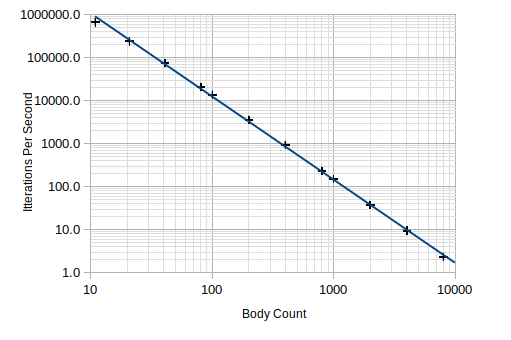
\includegraphics[width=0.9\textwidth]{img/testingEvidence/perfgraph1.png}
  \caption{Iterations/Second Over Body Count (Logarithmic)}
\end{figure}

\begin{figure}[!h]
  \centering
  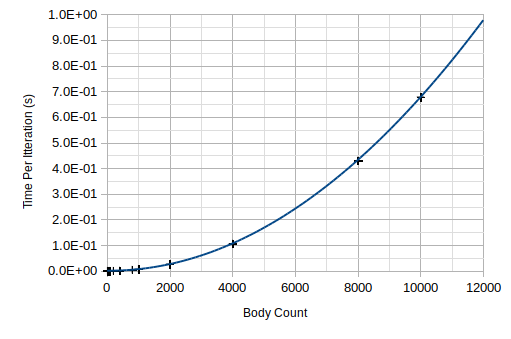
\includegraphics[width=0.9\textwidth]{img/testingEvidence/perfgraph2.png}
  \caption{Time/Iteration Over Body Count}
\end{figure}

\pagebreak

\subsubsection{SIM13}
SIM13 is a trace table based test which compares the results of the simulation between the intended algorithm being hand traced, in particular this trace table will compare results for the velocity and position of a single body.

\paragraph{}
The simulation in question contains two bodies, however in order to make the calculations more manageable one of the bodies is fixed, constantly residing at 0,0. A large time step of 2 (unit time) is specified, this allows for a quarter of an orbit to be completed in a single iteration, meaning that the change in numbers between iterations is of a manageable size and does not require a large number of significant figures to be kept.

\paragraph{}
The data calculated in the manual trace table and the program output can be found on the following pages. Comparing the two tables, the results match exactly when comparing the algorithm to a hand-run results.

\begin{figure}[h]
  \centering
  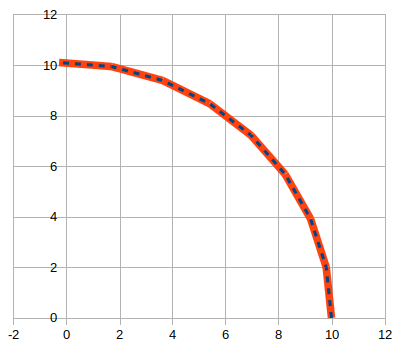
\includegraphics[width=0.8\textwidth]{img/testingEvidence/tracetable.png}
  \caption{Trace Table \& Program Output (Position)}
\end{figure}

\begin{table}[H]
\footnotesize
\centering
\caption{Manual Trace Table - 8 Iterations}
\def\arraystretch{1.4}
\begin{tabular}{|c|c|c|c|c|c|c|c|c|} \hline
Iteration & State    &   $p_x$ &  $p_y$ &  $v_x$ &  $v_y$ &  $a_x$ &  $a_y$ &  $r$   \\ \hline
0 & $Init$           &  10.000 &	0.000 &	 0.000 &	1.000 &	-0.100 &  0.000 & 10.000 \\ \hline
1 & $v\frac{1}{2}1$	 &  10.000 &  0.000 &	-0.100 &	1.000 &	-0.100 &  0.000 & -      \\ \hline
  & $r$	             &   9.800 &	2.000	& -0.100 & 	1.000	&	-	     & -      & -      \\ \hline
  & $a$	             &   9.800 &	2.000 &	-0.100 &	1.000 &	-0.098 & -0.020 &	10.002 \\ \hline
  & $v\frac{1}{2}2$	 &   9.800 &	2.000 &	-0.198 &	0.980 &	-0.098 & -0.020	& -      \\ \hline
2 & $v\frac{1}{2}1$	 &   9.800 &	2.000 &	-0.296 &	0.960 &	-0.098 & -0.020	& -      \\ \hline
  & $r$	             &   9.208 &	3.920 &	-0.296 &	0.960	&	-	     & -      & -      \\ \hline
  & $a$	             &   9.208 &	3.920 &	-0.296 &	0.960 &	-0.092 & -0.039 &	10.008 \\ \hline
  & $v\frac{1}{2}2$  &	 9.208 &	3.920 &	-0.388 &	0.921 &	-0.092 & -0.039	& -      \\ \hline
3 & $v\frac{1}{2}1$  &	 9.208 &	3.920	& -0.480 &	0.882 &	-0.092 & -0.039 &	-      \\ \hline
  & $r$              & 	 8.249 &	5.684	& -0.480 &	0.882 &	-		   & -      & -      \\ \hline
  & $a$              &	 8.249 &	5.684	& -0.480 &	0.882	& -0.082 & -0.057	& 10.017 \\ \hline
  & $v\frac{1}{2}2$  &	 8.249 &	5.684	& -0.562 &	0.825	& -0.082 & -0.057	& -      \\ \hline
4 & $v\frac{1}{2}1$  &	 8.249 &	5.684	& -0.644 &	0.769	& -0.082 & -0.057	& -      \\ \hline
  & $r$	             &   6.962 &	7.221	& -0.644 &	0.769	&	-	     & -      & -      \\ \hline
  & $a$              &   6.962 &	7.221	& -0.644 &	0.769	& -0.069 & -0.072 &	10.030 \\ \hline
  & $v\frac{1}{2}2$  &	 6.962 &	7.221 &	-0.713 &	0.697 &	-0.069 & -0.072	& -      \\ \hline
5 & $v\frac{1}{2}1$  &	 6.962 &	7.221 &	-0.782 &	0.626 &	-0.069 & -0.072	& -      \\ \hline
  & $r$	             &   5.398 &	8.472	& -0.782 &	0.626	&	-	     & -      & -      \\ \hline
  & $a$	             &   5.398 &	8.472	& -0.782 & 	0.626	& -0.053 & -0.084 &	10.046 \\ \hline
  & $v\frac{1}{2}2$  &	 5.398 &	8.472	& -0.835 &	0.542	& -0.053 & -0.084	& -      \\ \hline
6 & $v\frac{1}{2}1$	 &   5.398 &	8.472	& -0.888 &	0.458	& -0.053 & -0.084	& -      \\ \hline
  & $r$	             &   3.622 &	9.389	& -0.888 &	0.458	&	-	     & -      & -      \\ \hline
  & $a$	             &   3.622 &	9.389	& -0.888 &	0.458	& -0.036 & -0.092	& 10.064 \\ \hline
  & $v\frac{1}{2}2$  &	 3.622 & 	9.389	& -0.924 &	0.366	& -0.036 & -0.092	& -      \\ \hline
7 & $v\frac{1}{2}1$  &	 3.622 &	9.389	& -0.959 &	0.274	& -0.036 & -0.092	& -      \\ \hline
  & $r$	             &   1.703 &	9.938	& -0.959 &	0.274	& -		   & -      & -      \\ \hline
  & $a$	             &   1.703 &	9.938	& -0.959 &	0.274	& -0.017 & -0.097 &	10.083 \\ \hline
  & $v\frac{1}{2}2$  &	 1.703 &	9.938	& -0.976 &	0.177	& -0.017 & -0.097	& -      \\ \hline
8 & $v\frac{1}{2}1$  &	 1.703 &	9.938	& -0.992 &	0.080	& -0.017 & -0.097	& -      \\ \hline
  & $r$	             &  -0.282 & 10.098	& -0.992 &	0.080	&	-	     & -      & -      \\ \hline
  &	$a$              &  -0.282 & 10.098	& -0.992 &	0.080	&  0.003 & -0.098 &	10.102 \\ \hline
  & $v\frac{1}{2}2$  &	-0.282 & 10.098	& -0.990 & -0.018	&  0.003 & -0.098	& -      \\ \hline
\end{tabular}
\vspace{-40pt}
\end{table}

\pagebreak

\begin{table}[H]
\footnotesize
\centering
\caption{Program Output - 8 Iterations}
\def\arraystretch{1.5}
\begin{tabular}{|c|c|c|c|c|c|c|c|c|} \hline
Iteration & State    &   $p_x$ &  $p_y$ &  $v_x$ &  $v_y$ \\ \hline
0 & $Init$           &  10.000 &	0.000 &	 0.000 &	1.000 \\ \hline
1 & $v\frac{1}{2}1$	 &  10.000 &  0.000 &	-0.100 &	1.000 \\ \hline
  & $r$	             &   9.800 &	2.000	&  -     & 		    \\ \hline
  & $v\frac{1}{2}2$	 &   -     &	-     &	-0.198 &	0.980 \\ \hline
2 & $v\frac{1}{2}1$	 &   -     &	-     &	-0.296 &	0.960 \\ \hline
  & $r$	             &   9.208 &	3.920 &	 -     &	-    	\\ \hline
  & $v\frac{1}{2}2$  &	 -     &	-     &	-0.388 &	0.921 \\ \hline
3 & $v\frac{1}{2}1$  &	 -     &	-    	& -0.480 &	0.882 \\ \hline
  & $r$              & 	 8.249 &	5.684	&  -     &	-     \\ \hline
  & $v\frac{1}{2}2$  &	 -     &	-    	& -0.562 &	0.825	\\ \hline
4 & $v\frac{1}{2}1$  &	 -     &	-    	& -0.644 &	0.769	\\ \hline
  & $r$	             &   6.962 &	7.221	&  -     &	-    	\\ \hline
  & $v\frac{1}{2}2$  &	 -     &	-     &	-0.713 &	0.697 \\ \hline
5 & $v\frac{1}{2}1$  &	 -     &	-     &	-0.782 &	0.626 \\ \hline
  & $r$	             &   5.398 &	8.472	&  -     &	-    	\\ \hline
  & $v\frac{1}{2}2$  &	 -     &	-    	& -0.835 &	0.542	\\ \hline
6 & $v\frac{1}{2}1$	 &   -     &	-    	& -0.888 &	0.458	\\ \hline
  & $r$	             &   3.622 &	9.389	&  -     &	-    	\\ \hline
  & $v\frac{1}{2}2$  &	 -     & 	-    	& -0.924 &	0.366	\\ \hline
7 & $v\frac{1}{2}1$  &	 -     &	-    	& -0.959 &	0.274	\\ \hline
  & $r$	             &   1.703 &	9.938	&  -     &	-    	\\ \hline
  & $v\frac{1}{2}2$  &	 -     &	-    	& -0.976 &	0.177	\\ \hline
8 & $v\frac{1}{2}1$  &	 -     &	-    	& -0.992 &	0.080	\\ \hline
  & $r$	             &  -0.282 & 10.098	&  -     &	-    	\\ \hline
  & $v\frac{1}{2}2$  &	 -     &  -    	& -0.990 & -0.018	\\ \hline
\end{tabular}
\vspace{-40pt}
\end{table}

\pagebreak

\subsubsection{SIM19}
SIM19 is another trace table based test where the algorithm for the calculation of every force acting on each pair of bodies is compared to the results given by the simulation. This algorithm is the main algorithm that was changed from the initial design documentation, relying solely on a offset double for loop to calculate the relationships between every body in the simulation, yet miss out the calculations which are unnecessary. (Highlighted by the initial use of a matrix like algorithm.)

\paragraph{}
Comparing the outputs, the trace tables show the same final results for each force and all of the forces intended to be calculated were calculated.

\begin{table}[H]
\footnotesize
\centering
\caption{Trace Table - 6 Bodies}
\def\arraystretch{1.5}
\begin{tabular}{|c|c|c|c|c|c|c|c|c|c|c|} \hline
$x$ & $y$ & $p_{xA}$ & $p_{yA}$ & $p_{xB}$ & $p_{yB}$ & $r_x$ & $r_y$ & $r$ & $F_x$ & $F_y$ \\ \hline
0	& 1 &	 10 &   2 &	 -4 &	  4 &	 14 &	 -2 &	14.14 &	\textbf{-0.0495} & \textbf{ 0.0071} \\ \hline
0	& 2	&  10	&   2 & -18 &	 16	&  28 &	-14	& 31.30	& \textbf{-0.0091} & \textbf{ 0.0046} \\ \hline
0	& 3	&  10	&   2 &  -8 &	-12	&  18	&  14	& 22.80	& \textbf{-0.0152} & \textbf{-0.0118} \\ \hline
0	& 4	&  10	&   2 &   6 & -13	&   4	&  15	& 15.52	& \textbf{-0.0107} & \textbf{-0.0401} \\ \hline
0	& 5	&  10	&   2 &   8 &  11	&   2	&  -9	&  9.22	& \textbf{-0.0255} & \textbf{ 0.1148} \\ \hline
1	& 2	&  -4	&   4 &	-18 &	 16	&  14	& -12	& 18.44	& \textbf{-0.0223} & \textbf{ 0.0191} \\ \hline
1	& 3	&  -4	&   4 &  -8 &	-12	&   4	&  16	& 16.49	& \textbf{-0.0089} & \textbf{-0.0357} \\ \hline
1	& 4	&  -4	&   4 &   6 &	-13	& -10	&  17	& 19.72	& \textbf{ 0.0130} & \textbf{-0.0222} \\ \hline
1	& 5	&  -4	&   4 &	  8 &  11	& -12	&  -7	& 13.89	& \textbf{ 0.0448} & \textbf{ 0.0261} \\ \hline
2	& 3	& -18	&  16	&  -8 &	-12	& -10	&  28	& 29.73	& \textbf{ 0.0038} & \textbf{-0.0107} \\ \hline
2	& 4	& -18	&  16	&   6 & -13	& -24	&  29	& 37.64	& \textbf{ 0.0045} & \textbf{-0.0054} \\ \hline
2	& 5	& -18	&  16	&   8 &  11	& -26	&   5	& 26.48	& \textbf{ 0.0140} & \textbf{-0.0027} \\ \hline
3	& 4	&  -8	& -12	&   6 & -13	& -14	&   1	& 14.04	& \textbf{ 0.0506} & \textbf{-0.0036} \\ \hline
3	& 5	&  -8	& -12	&   8 &  11	& -16	& -23	& 28.02	& \textbf{ 0.0073} & \textbf{ 0.0105} \\ \hline
4	& 5	&   6	& -13 &	  8 &  11 &	 -2	& -24	& 24.08 &	\textbf{ 0.0014} & \textbf{ 0.0172} \\ \hline
\end{tabular}
\vspace{-40pt}
\end{table}

\pagebreak

\begin{table}[H]
\footnotesize
\centering
\caption{Program Output - 6 Bodies}
\def\arraystretch{1.5}
\begin{tabular}{|c|c|c|c|} \hline
$x$ & $y$ & $F_x$ & $F_y$ \\ \hline
0 & 1	&	\textbf{-0.0495} & \textbf{ 0.0071} \\ \hline
0 & 2	&	\textbf{-0.0091} & \textbf{ 0.0046} \\ \hline
0 & 3	&	\textbf{-0.0152} & \textbf{-0.0118} \\ \hline
0 & 4	&	\textbf{-0.0107} & \textbf{-0.0401} \\ \hline
0 & 5	&	\textbf{-0.0255} & \textbf{ 0.1148} \\ \hline
1 & 2	&	\textbf{-0.0223} & \textbf{ 0.0191} \\ \hline
1 & 3	&	\textbf{-0.0089} & \textbf{-0.0357} \\ \hline
1 & 4	& \textbf{ 0.0130} & \textbf{-0.0222} \\ \hline
1 & 5	&	\textbf{ 0.0448} & \textbf{ 0.0261} \\ \hline
2 & 3	&	\textbf{ 0.0038} & \textbf{-0.0107} \\ \hline
2 & 4	&	\textbf{ 0.0045} & \textbf{-0.0054} \\ \hline
2 & 5	&	\textbf{ 0.0140} & \textbf{-0.0027} \\ \hline
3 & 4	&	\textbf{ 0.0506} & \textbf{-0.0036} \\ \hline
3 & 5	&	\textbf{ 0.0073} & \textbf{ 0.0105} \\ \hline
4 & 5	&	\textbf{ 0.0014} & \textbf{ 0.0172} \\ \hline
\end{tabular}
\end{table}

\subsection{Videos}
Some evidence of testing has been provided in the form of video in order to make the results of certain tests clearer, as it would be difficult to adequately provide the change in information in a still image. The video evidence was for simulation tests only. (See provided CD) The following tests have video evidence provided.

\begin{itemize}
\item SIM4
\item SIM6
\item SIM8 - Video of Failure
\item SIM10 - Modified scenario, collisions on to show frame-rate variance.
\item SIM11
\item SIM12
\item SIM14
\item SIM15
\item SIM16
\item SIM17
\end{itemize}

\subsection{Screenshots and Logs}
\subsubsection{System Tests}
\begin{figure}[h]
  \centering
  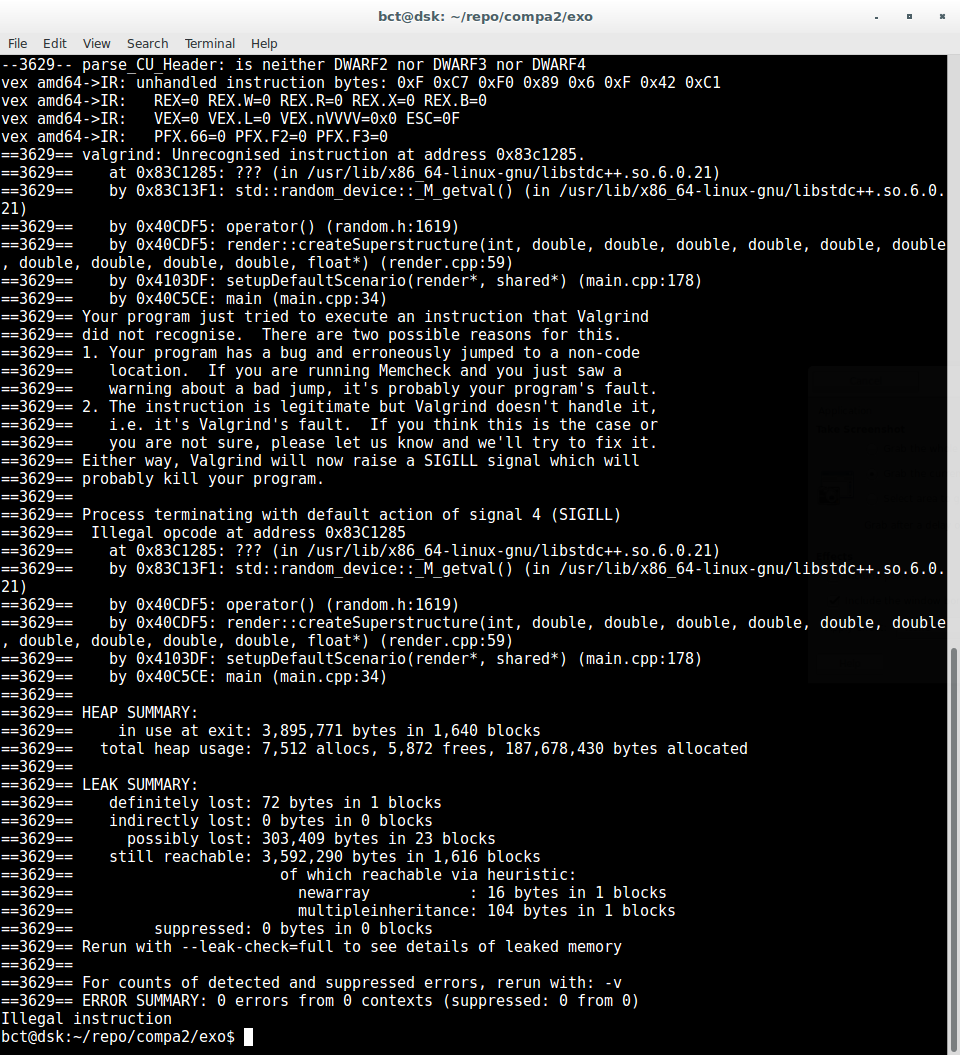
\includegraphics[width=0.9\textwidth]{img/testingEvidence/sys1rdcrash.png}
  \caption{SYS1 - Valgrind Fail}
\end{figure}
\begin{figure}[H]
  \centering
  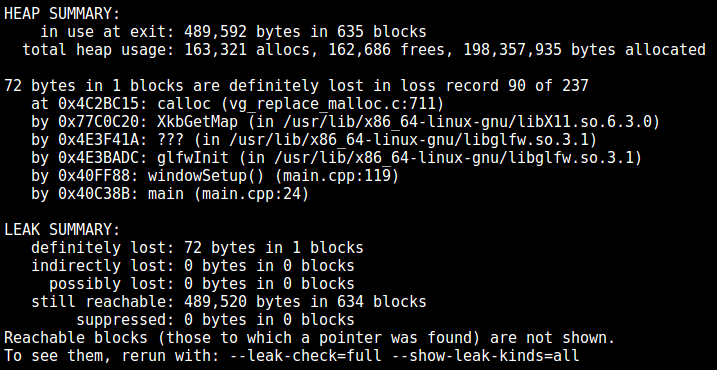
\includegraphics[width=\textwidth]{img/testingEvidence/glfwleak.png}
  \caption{SYS1 - GLFW Leak Details}
\end{figure}
\paragraph{}
The 72 Byte leak appears to be related to code in the GLFW library, as it is memory allocated by the \textit{glfwInit} function when the program starts up. The reference also pertains to the Linux display manager \textit{X11}, which could mean that this leak is Linux specific, extra testing should be carried out when the application is ported to a Windows system.

\pagebreak

\lstinputlisting[language={}, title=SYS1 - Valgrind Log]{img/testingEvidence/sys1.log}

\lstinputlisting[language={}, title=SYS2 - Valgrind Log]{img/testingEvidence/sys2.log}

\pagebreak

\begin{figure}[H]
  \centering
  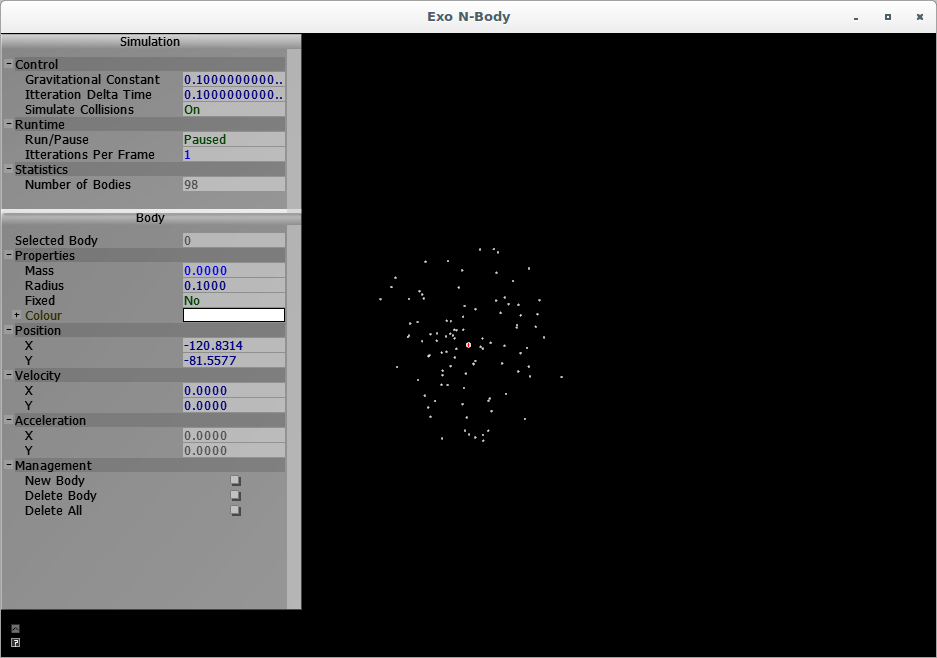
\includegraphics[width=0.85\textwidth]{img/testingEvidence/sys2_0.png}
  \caption{SYS2 - Initial}
\end{figure}

\begin{figure}[H]
  \centering
  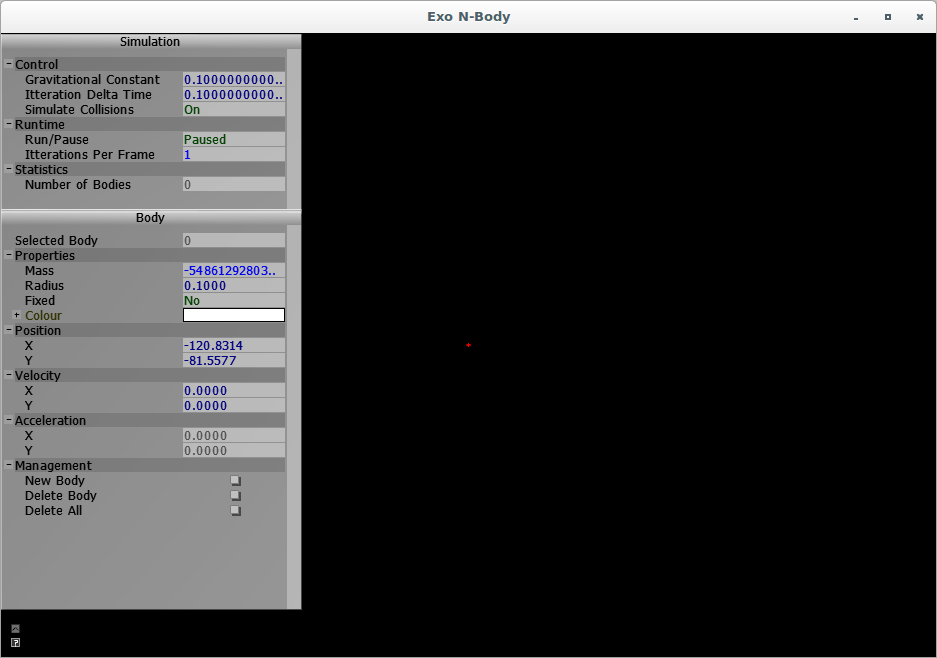
\includegraphics[width=0.85\textwidth]{img/testingEvidence/sys2_1.png}
  \caption{SYS2 - After Delete (Remaining numbers due to Valgrind issue.)}
\end{figure}

\pagebreak

\lstinputlisting[language={}, title=SYS3 - Valgrind Log]{img/testingEvidence/sys3.log}

\begin{figure}[H]
  \centering
  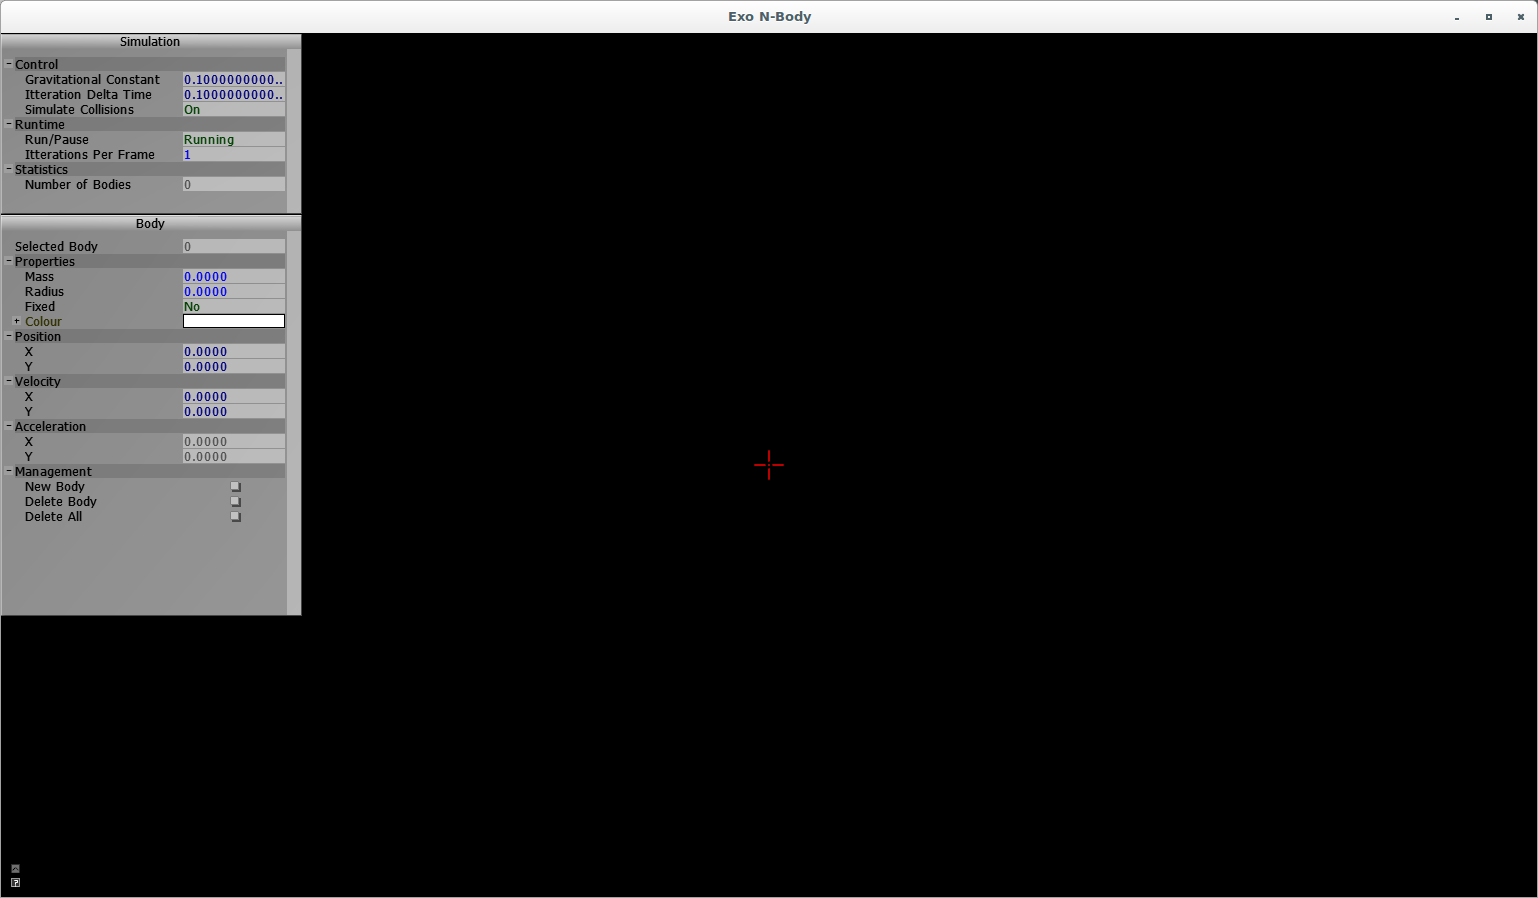
\includegraphics[width=\textwidth]{img/testingEvidence/sys3_0.png}
  \caption{SYS3 - Initial}
\end{figure}

\begin{figure}[H]
  \centering
  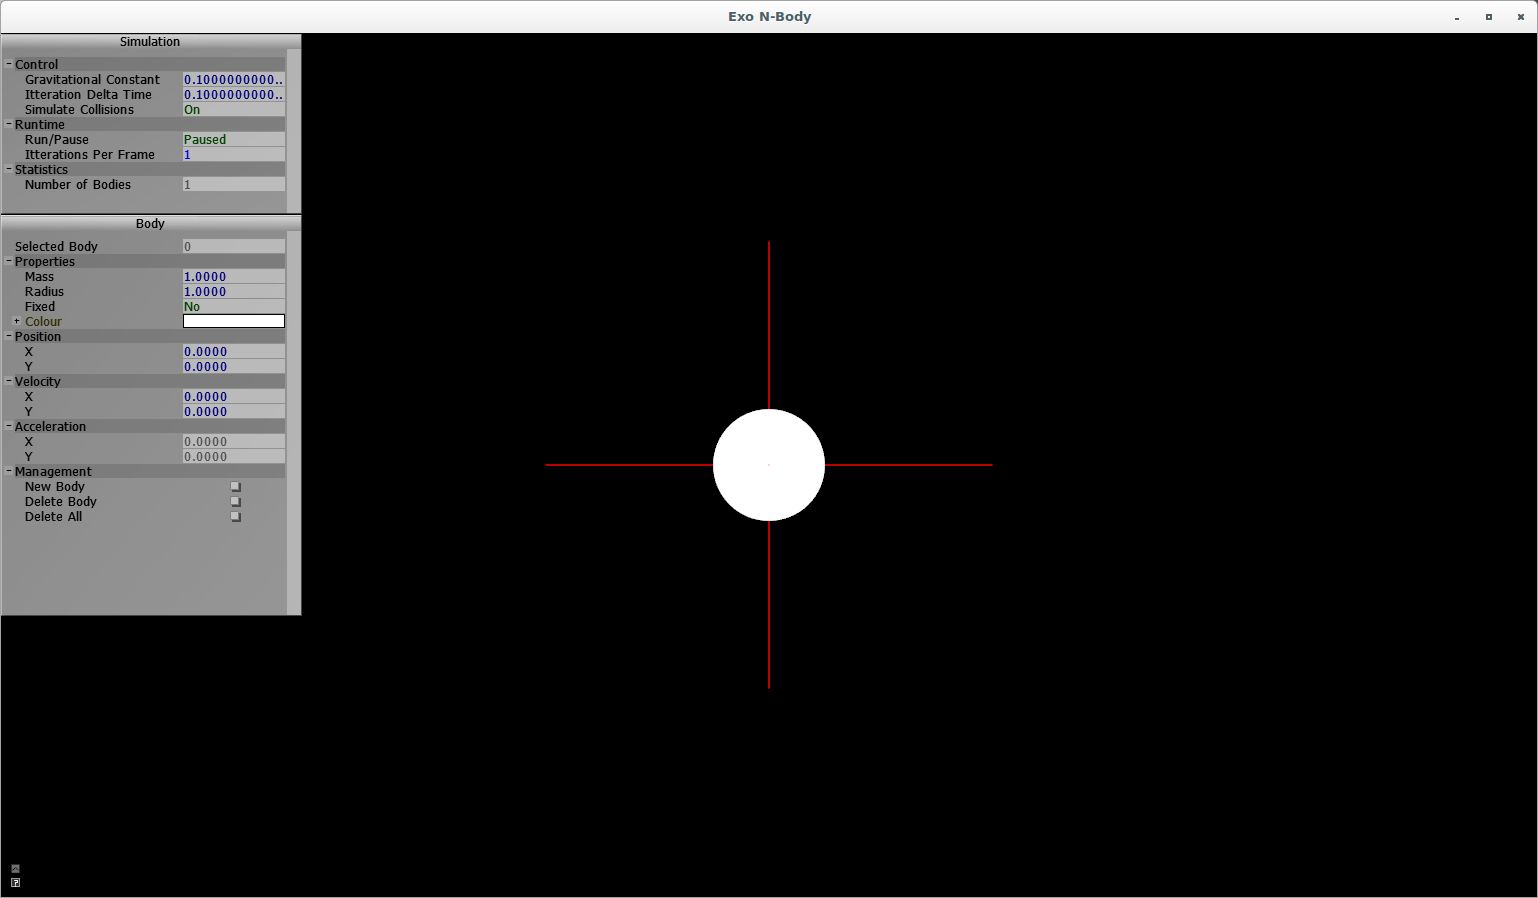
\includegraphics[width=\textwidth]{img/testingEvidence/sys3_1.png}
  \caption{SYS3 - After Placement}
\end{figure}

\lstinputlisting[language={}, title=SYS4 - Valgrind Log]{img/testingEvidence/sys4.log}

\pagebreak

\begin{figure}[H]
  \centering
  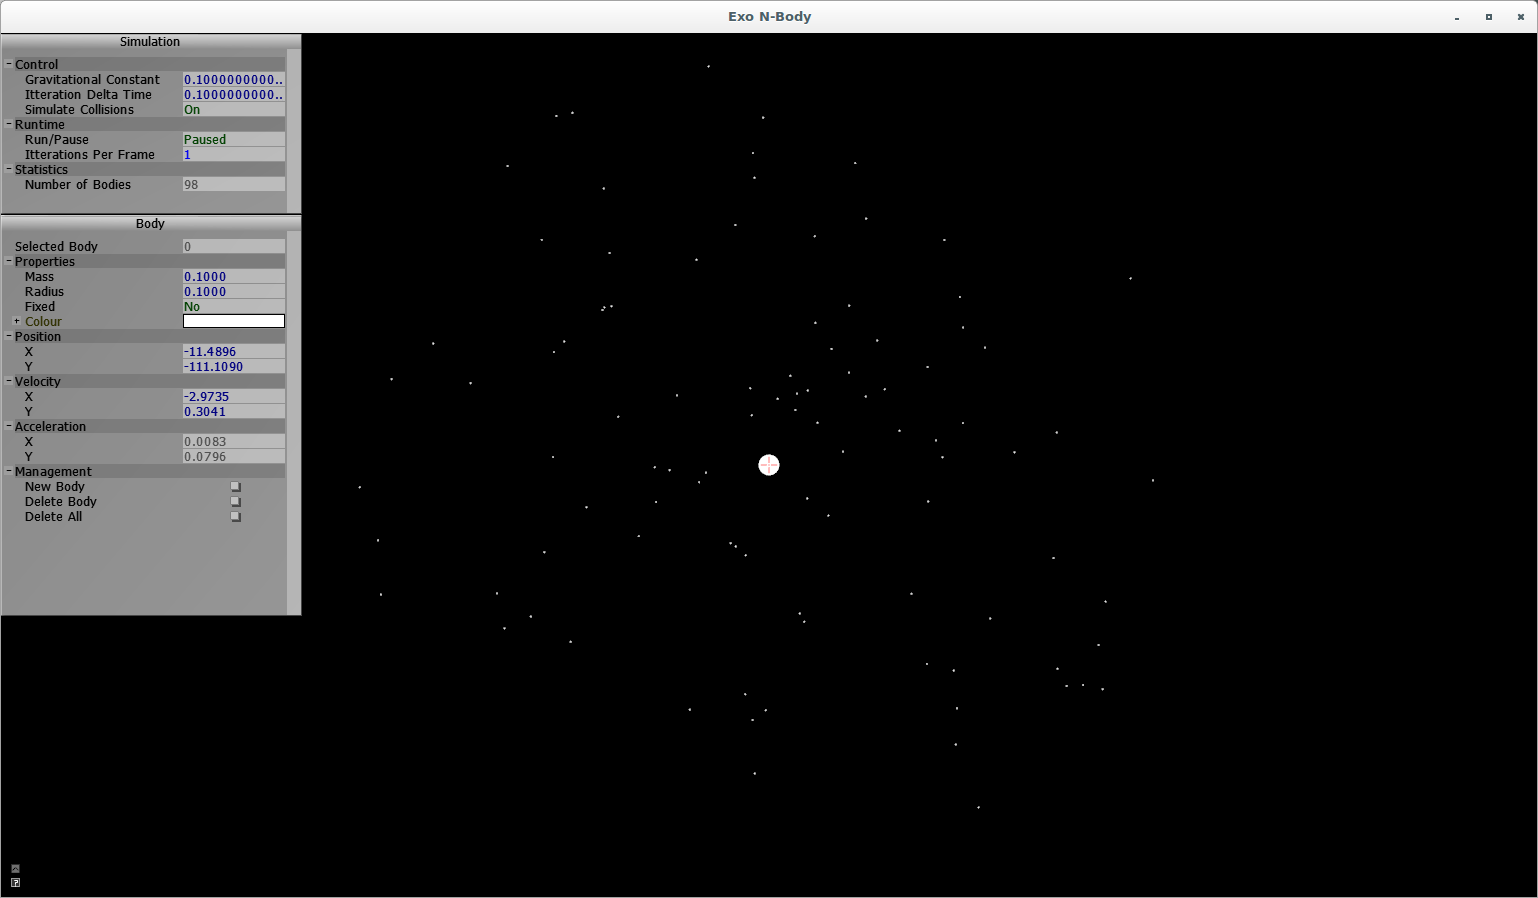
\includegraphics[width=\textwidth]{img/testingEvidence/sys4_0.png}
  \caption{SYS4 - Initial}
\end{figure}

\begin{figure}[H]
  \centering
  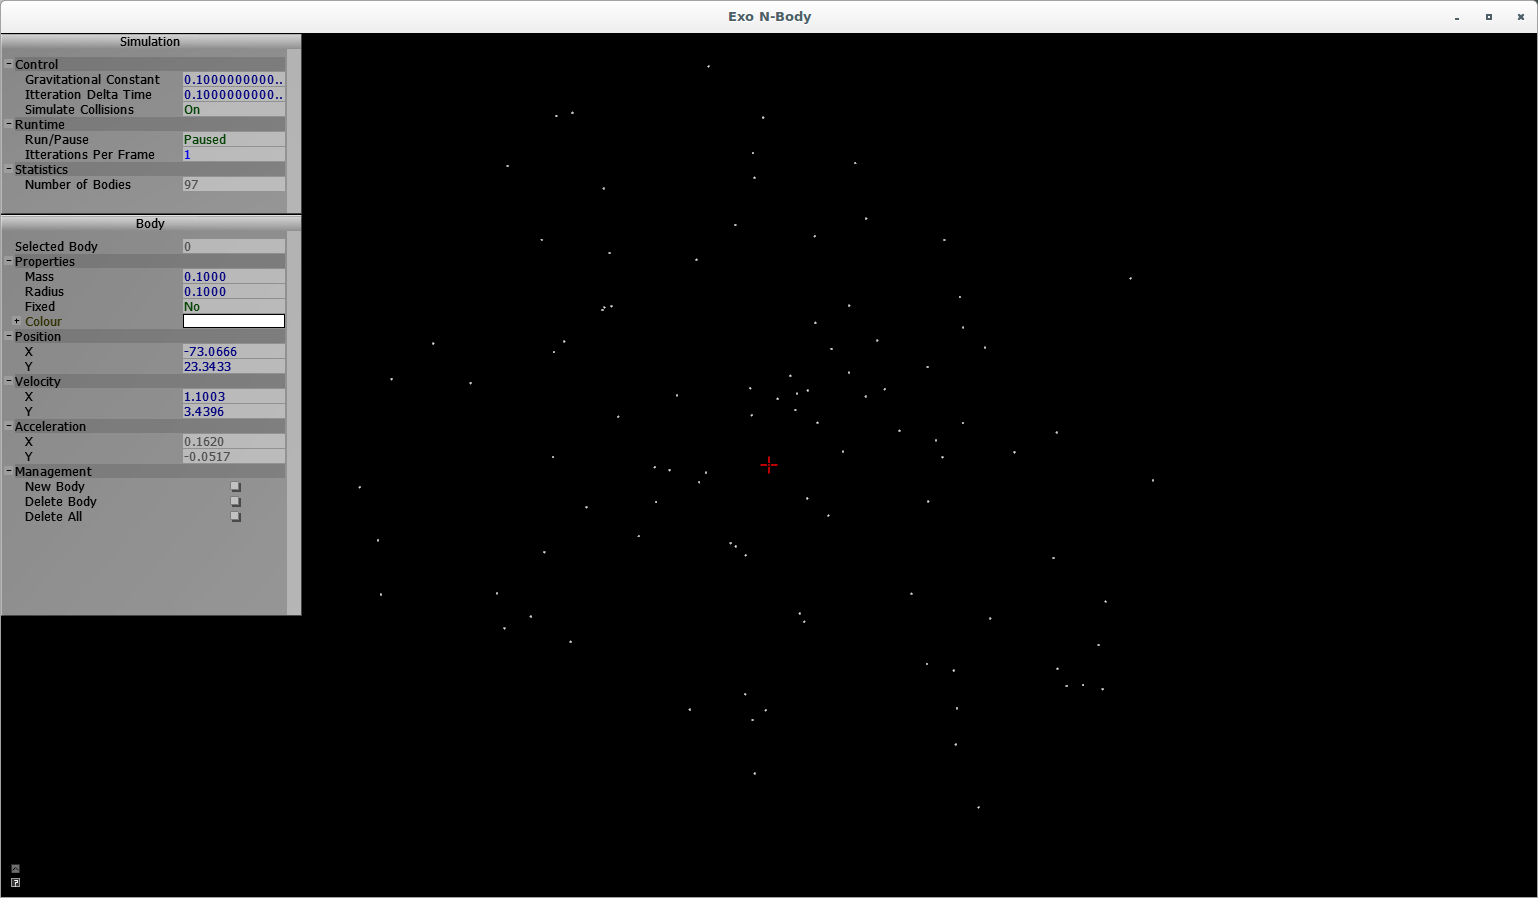
\includegraphics[width=\textwidth]{img/testingEvidence/sys4_1.png}
  \caption{SYS4 - After Delete}
\end{figure}

\pagebreak

\begin{figure}[H]
  \centering
  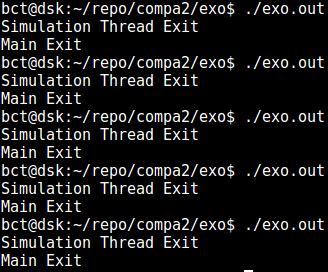
\includegraphics[width=0.5\textwidth]{img/testingEvidence/sys5.png}
  \caption{SYS5 - Exit Synchronisation}
\end{figure}

\lstinputlisting[language={}, title=SYS6 - Helgrind Log]{img/testingEvidence/sys6.log}

\paragraph{}
The errors in this log seem to pertain to the \textit{control\_variable}, which is an C++ STL class type which is used in the shared class, I believe these errors pertain to the variable not having an associated mutex lock until the simulation thread has correctly started, as the errors do not occur during runtime.

\pagebreak

\subsubsection{Interface Tests}
\begin{figure}[H]
  \centering
  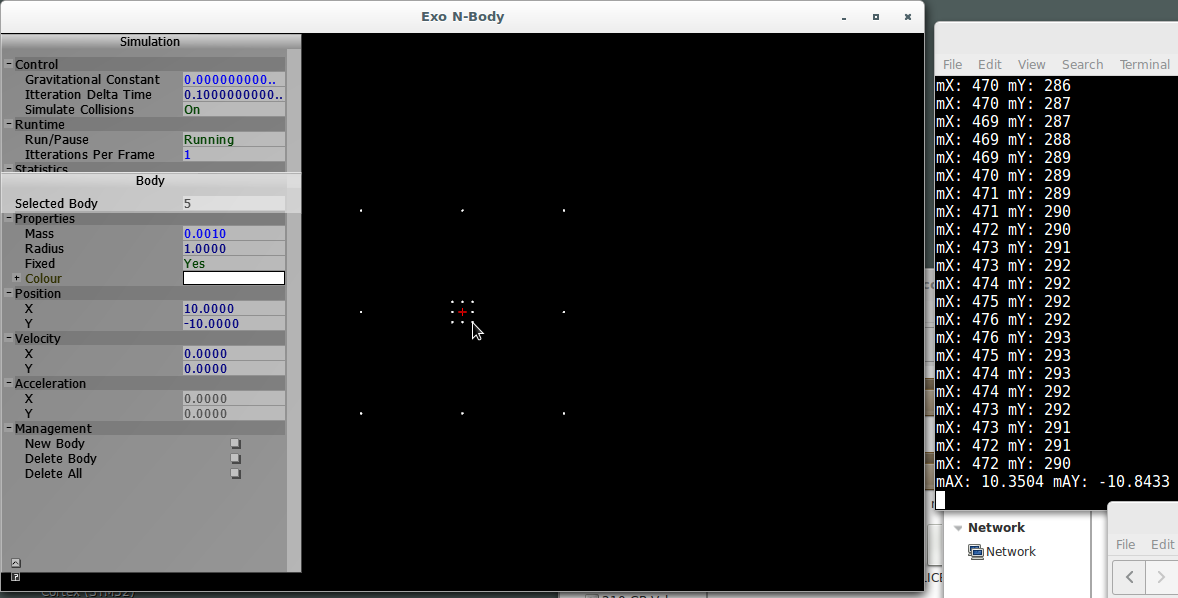
\includegraphics[width=\textwidth]{img/testingEvidence/gui1_0.png}
  \caption{GUI1 - [10,-10]}
\end{figure}

\begin{figure}[H]
  \centering
  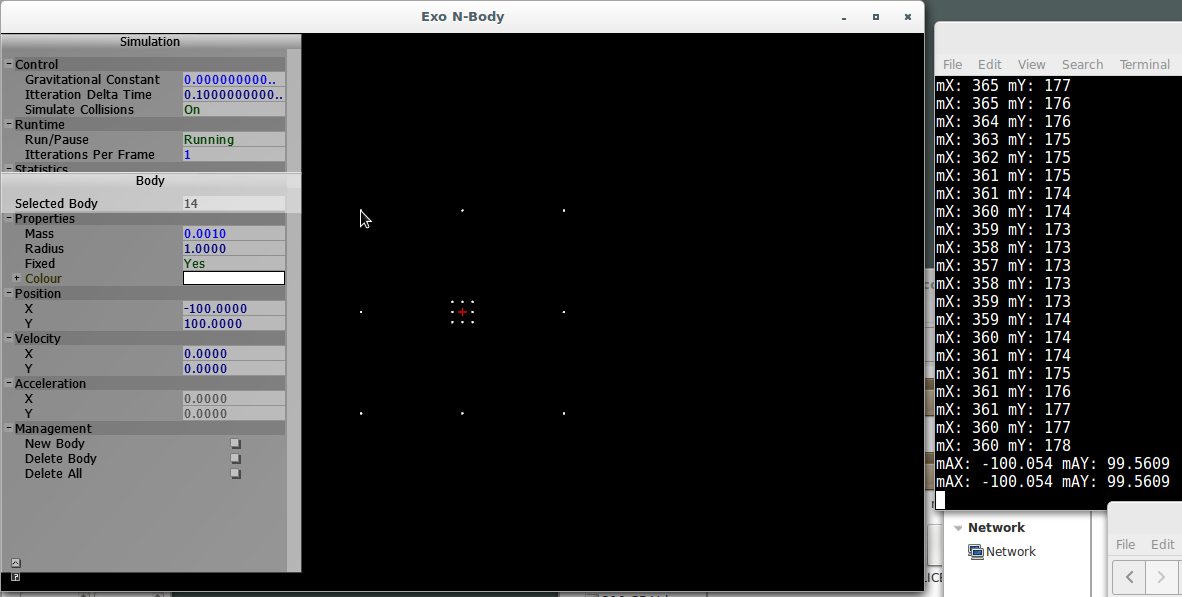
\includegraphics[width=\textwidth]{img/testingEvidence/gui1_1.png}
  \caption{GUI1 - [-100,100]}
\end{figure}

\pagebreak

\begin{figure}[H]
  \centering
  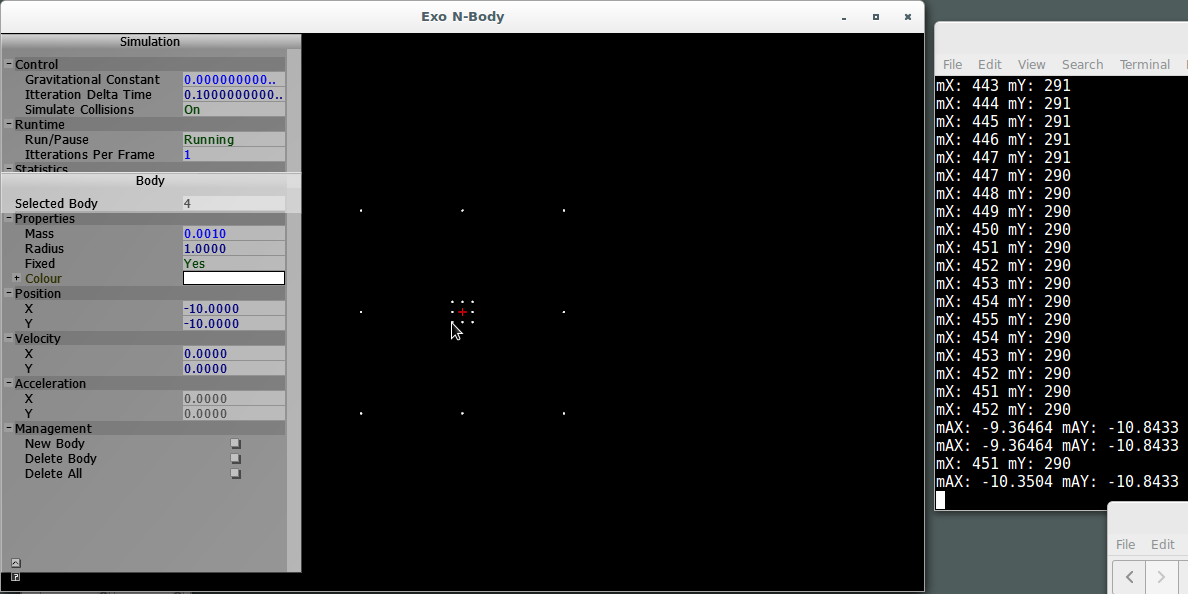
\includegraphics[width=\textwidth]{img/testingEvidence/gui1_2.png}
  \caption{GUI1 - [-10,-10]}
\end{figure}

\begin{figure}[H]
  \centering
  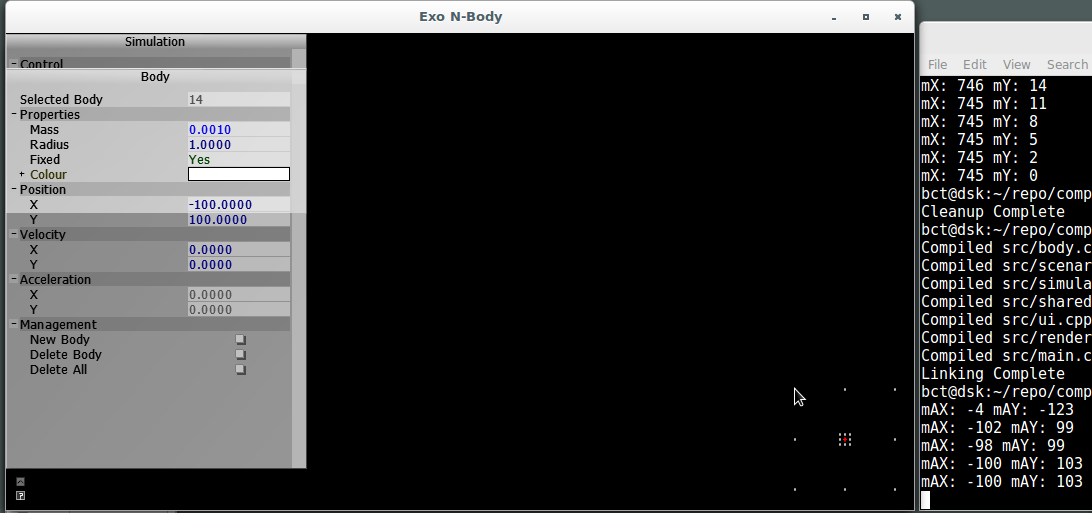
\includegraphics[width=\textwidth]{img/testingEvidence/gui2_0.png}
  \caption{GUI2 - [-100,100] with upper left pan.}
\end{figure}

\pagebreak

\begin{figure}[H]
  \centering
  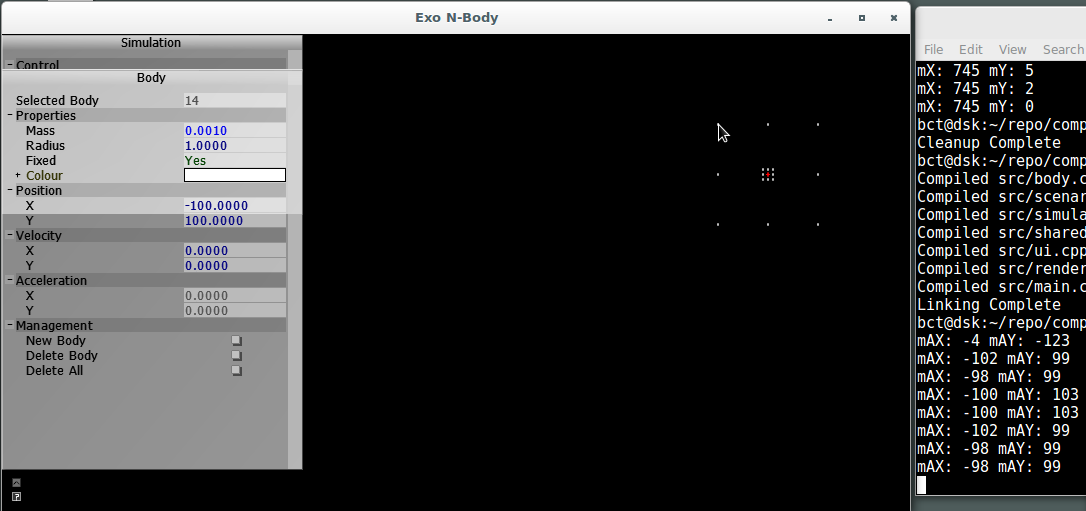
\includegraphics[width=\textwidth]{img/testingEvidence/gui2_1.png}
  \caption{GUI1 - [-100,100] with lower left pan.}
\end{figure}

\begin{figure}[H]
  \centering
  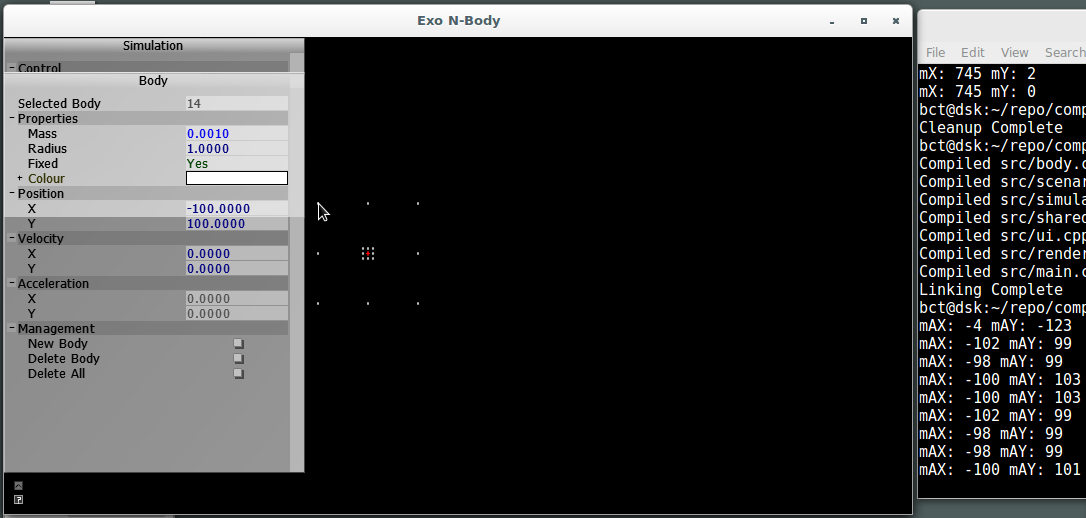
\includegraphics[width=\textwidth]{img/testingEvidence/gui2_2.png}
  \caption{GUI2 - [-100,100] with central right pan.}
\end{figure}

\pagebreak

\begin{figure}[H]
  \centering
  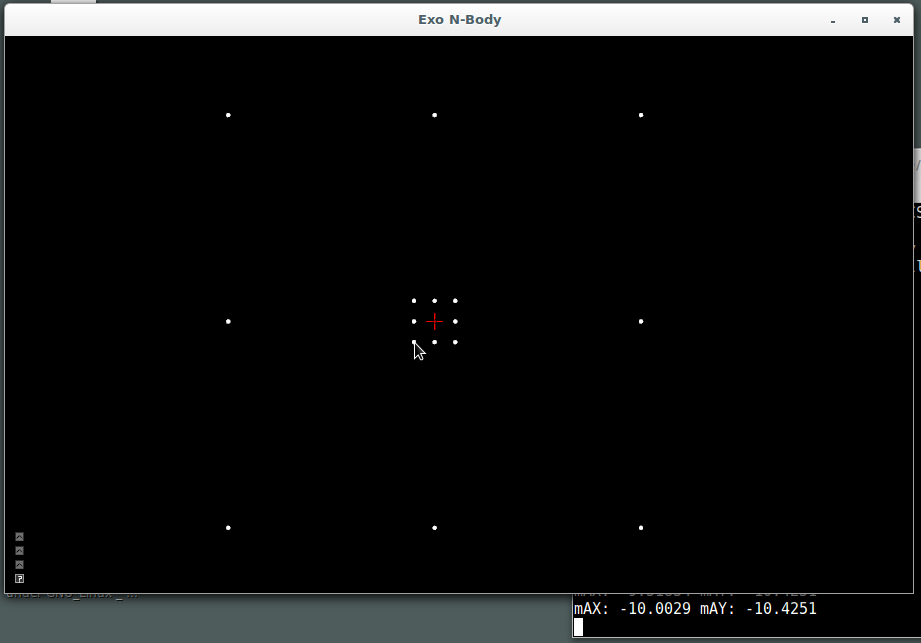
\includegraphics[width=0.85\textwidth]{img/testingEvidence/gui3_0.png}
  \caption{GUI3 - [-10,-10] with zoom in.}
\end{figure}

\begin{figure}[H]
  \centering
  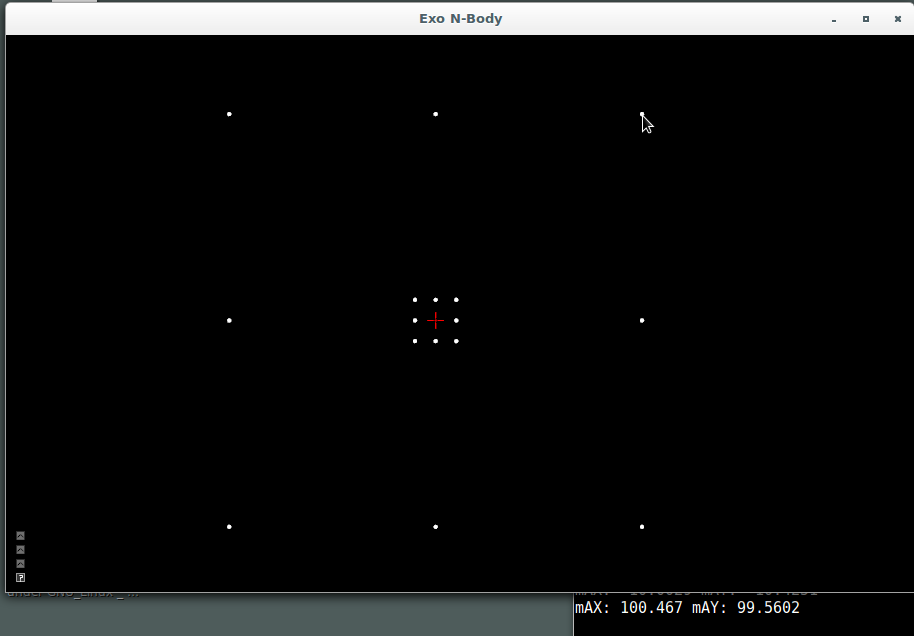
\includegraphics[width=0.85\textwidth]{img/testingEvidence/gui3_1.png}
  \caption{GUI3 - [100,100] with zoom in.}
\end{figure}

\begin{figure}[H]
  \centering
  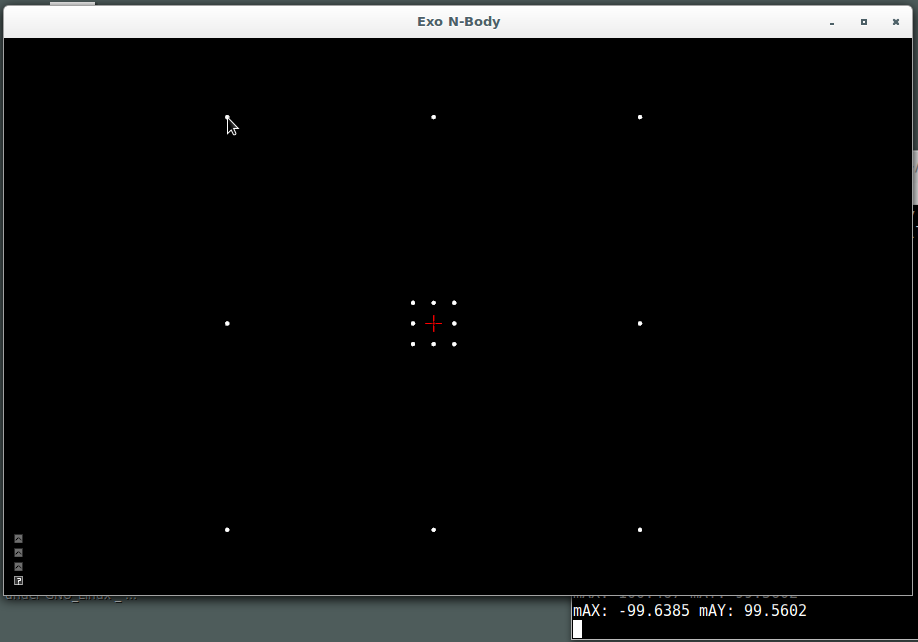
\includegraphics[width=0.85\textwidth]{img/testingEvidence/gui3_2.png}
  \caption{GUI3 - [-100,100] with zoom in.}
\end{figure}

\begin{figure}[H]
  \centering
  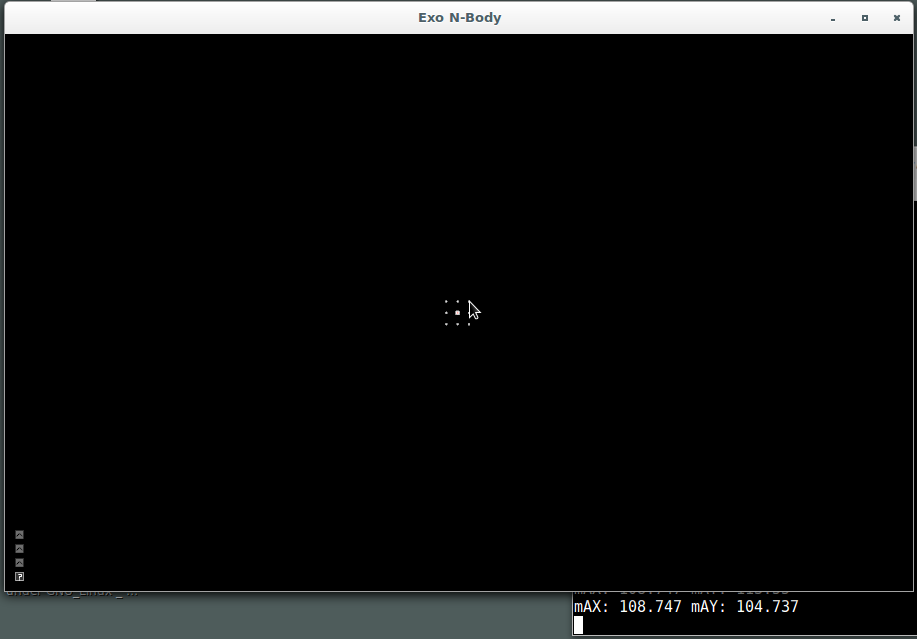
\includegraphics[width=0.85\textwidth]{img/testingEvidence/gui3_3.png}
  \caption{GUI3 - [100,100] with zoom out.}
\end{figure}

\begin{figure}[H]
  \centering
  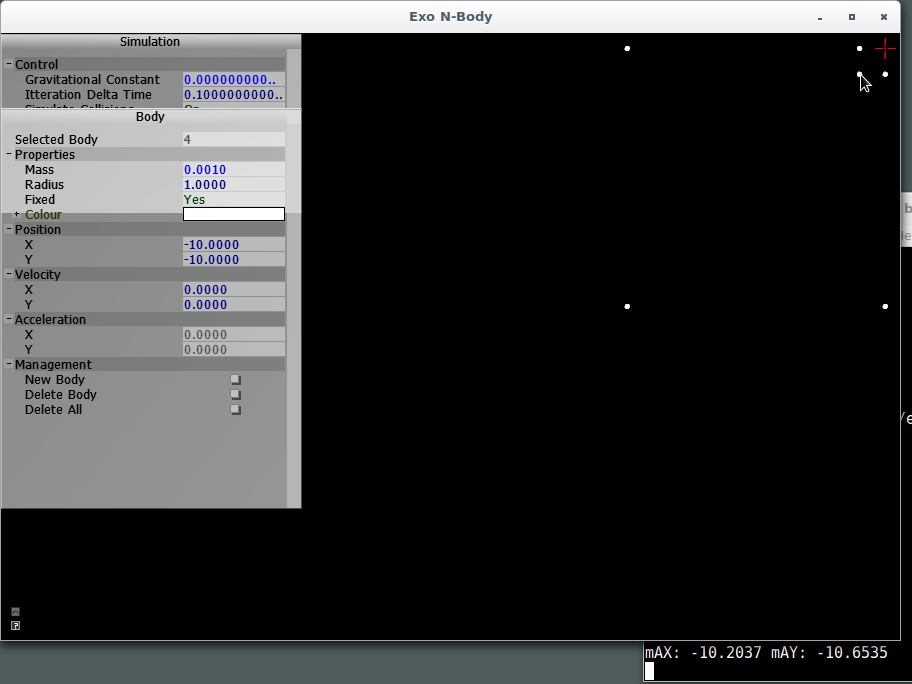
\includegraphics[width=0.8\textwidth]{img/testingEvidence/gui4.png}
  \caption{GUI4 - [-10,-10] with zoom in and lower left pan.}
\end{figure}

\begin{figure}[H]
  \centering
  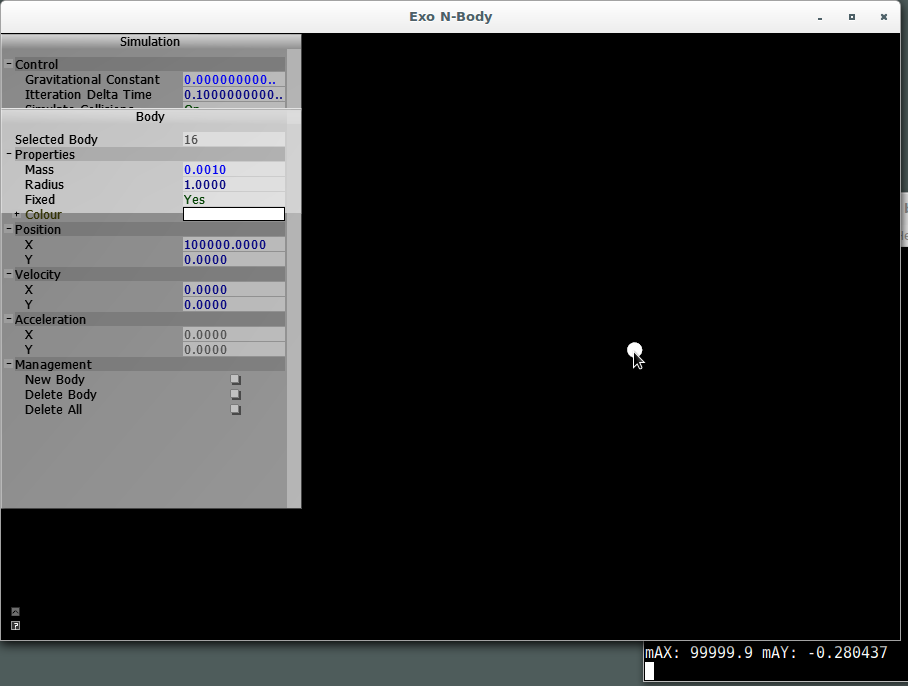
\includegraphics[width=0.8\textwidth]{img/testingEvidence/gui5.png}
  \caption{GUI5 - [1E5,0] Extreme selection.}
\end{figure}

\begin{figure}[H]
  \centering
  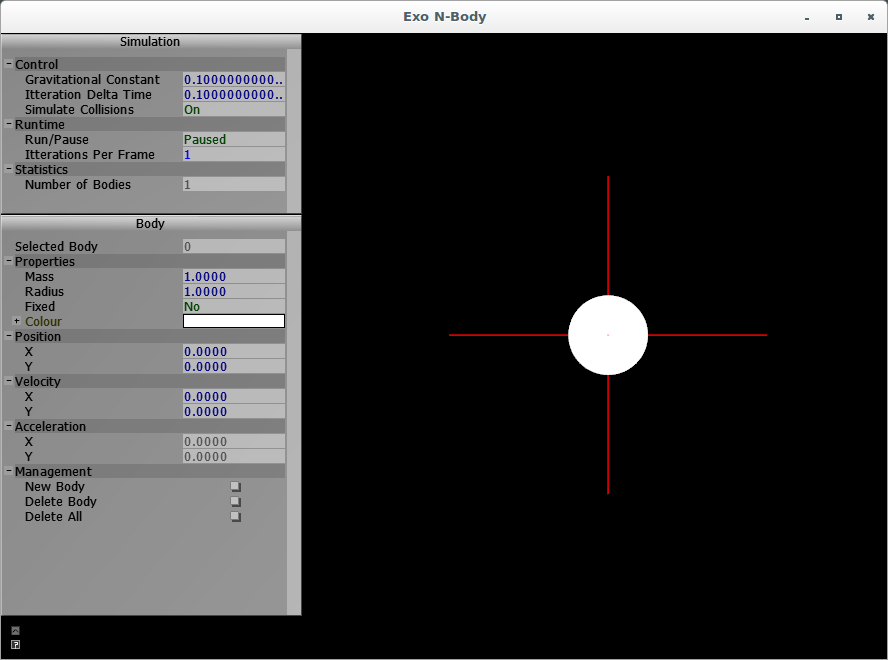
\includegraphics[width=0.8\textwidth]{img/testingEvidence/gui6.png}
  \caption{GUI6 - Body Add. (GUI)}
\end{figure}

\begin{figure}[H]
  \centering
  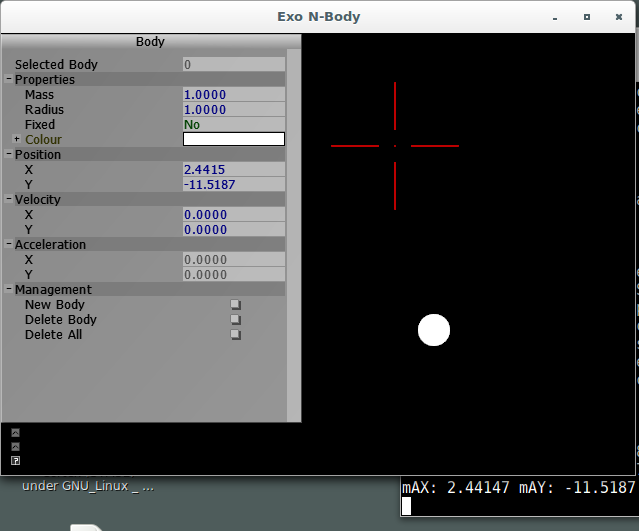
\includegraphics[width=0.75\textwidth]{img/testingEvidence/gui7.png}
  \caption{GUI7 - Body Add. (Mouse)}
\end{figure}

\begin{figure}[H]
  \centering
  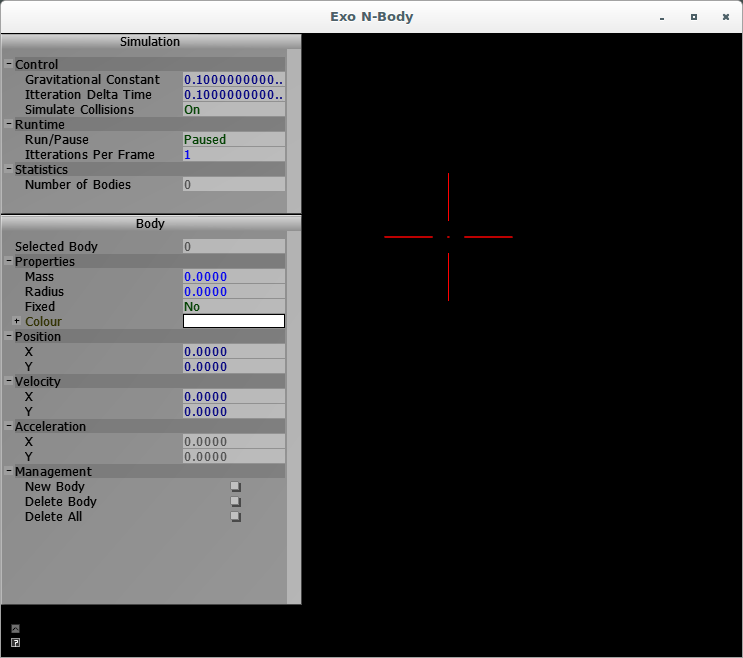
\includegraphics[width=0.7\textwidth]{img/testingEvidence/gui8.png}
  \caption{GUI8 - Body Delete.}
\end{figure}

\begin{figure}[H]
  \centering
  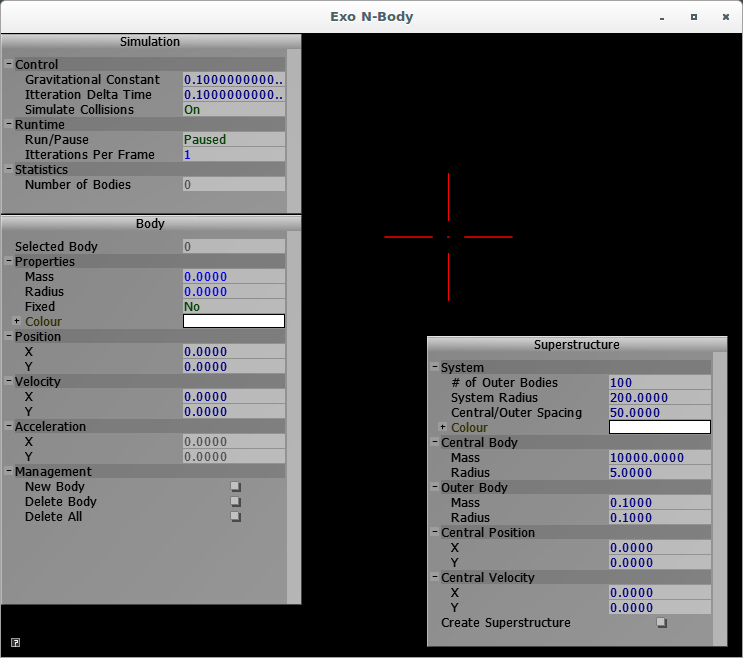
\includegraphics[width=0.7\textwidth]{img/testingEvidence/gui11.png}
  \caption{GUI11 - Opened Superstructure Creation Window.}
\end{figure}

\begin{figure}[H]
  \centering
  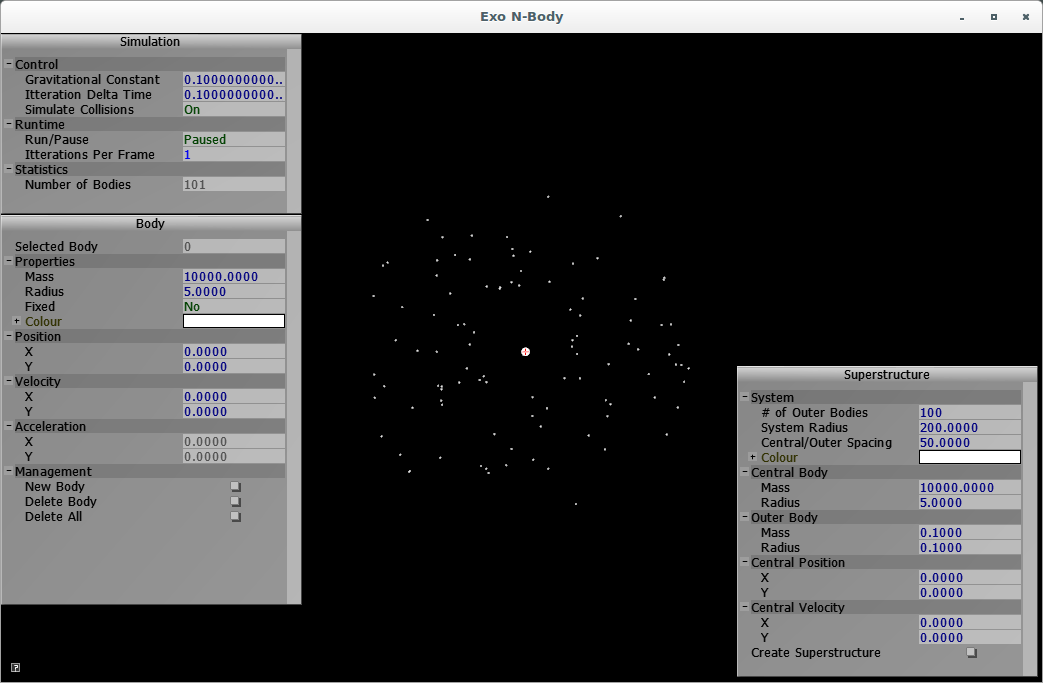
\includegraphics[width=0.8\textwidth]{img/testingEvidence/gui12.png}
  \caption{GUI12 - Superstructure Created.}
\end{figure}

\begin{wrapfigure}{hr}{0.5\textwidth}
  \centering
  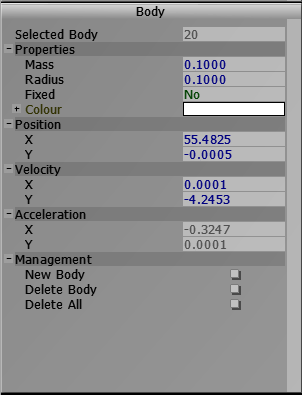
\includegraphics[width=0.45\textwidth]{img/testingEvidence/gui13.png}
  \caption{GUI13 - Superstructure Body Orbital Velocity.}
  \vspace{-10pt}
\end{wrapfigure}
\textbf{SIM13 Check:} \\\\
Body is orbiting at radius 55.4825. \\\\
It has a velocity in $y$ of -4.2453. \\\\
It has a mass of 0.1. \\\\
It is orbiting a mass of 10000. \\\\
The gravitational constant is 0.1. \\\\

$$\sqrt{\frac{0.1(10000+0.1)}{55.4825}} = 4.2455$$ \\\\

\pagebreak

\begin{figure}[H]
  \centering
  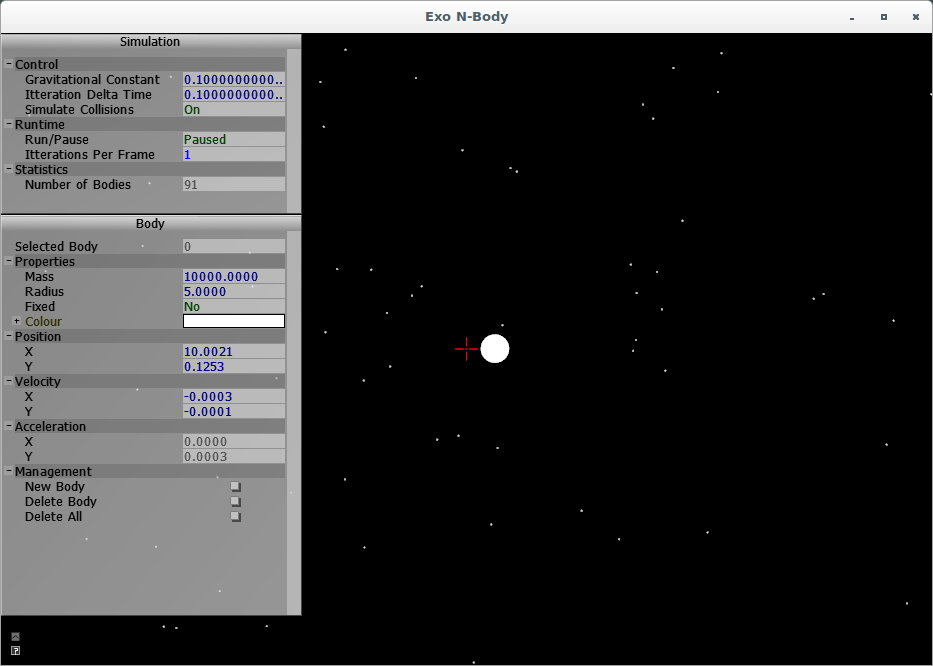
\includegraphics[width=0.8\textwidth]{img/testingEvidence/gui14_0.png}
  \caption{GUI14 - Initial State.}
\end{figure}

\begin{figure}[H]
  \centering
  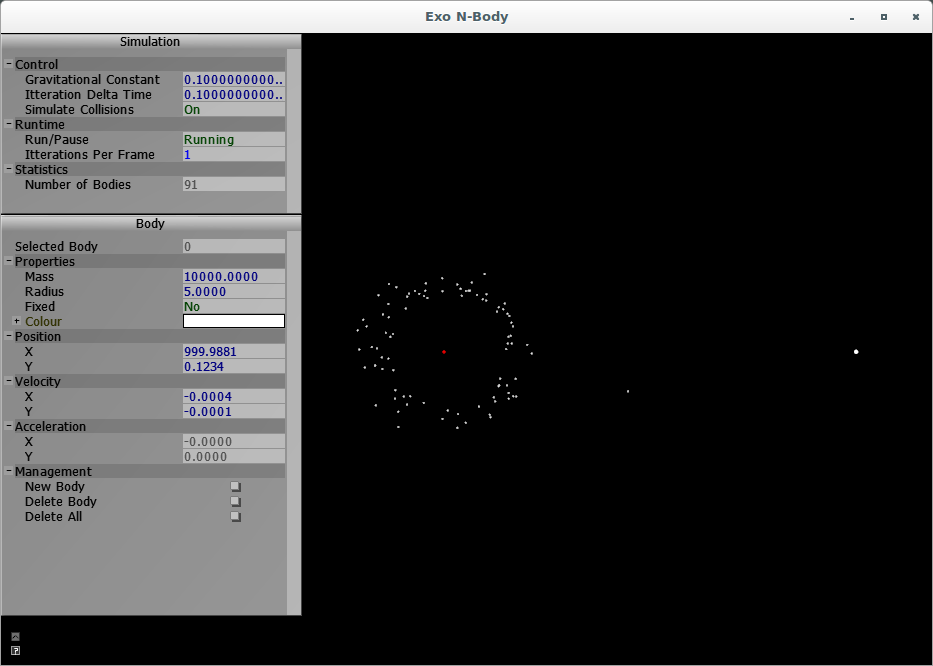
\includegraphics[width=0.8\textwidth]{img/testingEvidence/gui14_1.png}
  \caption{GUI14 - Body Position Changed.}
\end{figure}

\begin{figure}[H]
  \centering
  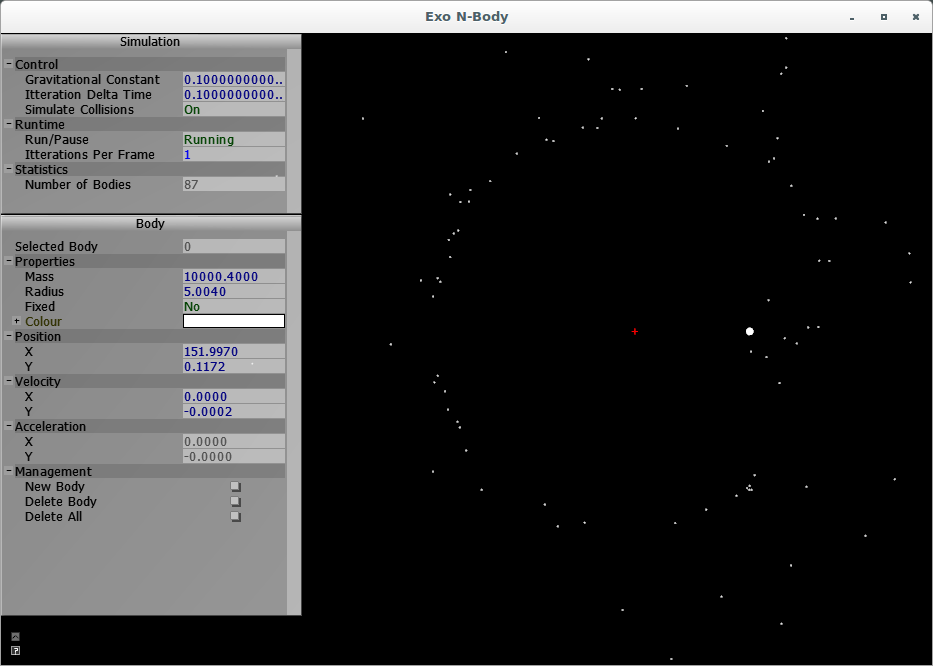
\includegraphics[width=0.8\textwidth]{img/testingEvidence/gui14_2.png}
  \caption{GUI14 - Body Position Changed.}
\end{figure}

\begin{figure}[H]
  \centering
  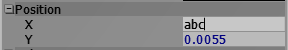
\includegraphics[width=0.8\textwidth]{img/testingEvidence/gui15_0.png}
  \caption{GUI15 - Erroneous AntTweakBar Value.}
\end{figure}

\begin{figure}[H]
  \centering
  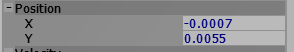
\includegraphics[width=0.8\textwidth]{img/testingEvidence/gui15_1.png}
  \caption{GUI15 - Erroneous AntTweakBar Value Not Accepted.}
\end{figure}

\pagebreak

\begin{figure}[H]
  \centering
  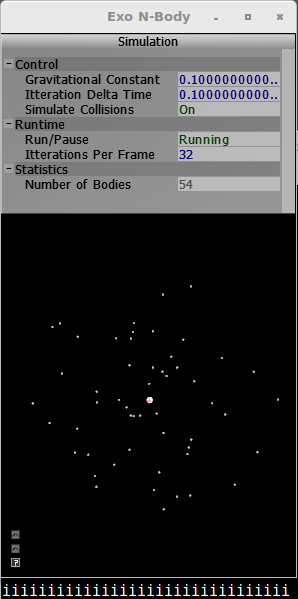
\includegraphics[width=0.6\textwidth]{img/testingEvidence/gui16_3.png}
  \caption{GUI16 - 32 Iterations per Frame.}
\end{figure}

\pagebreak

\begin{figure}[H]
  \centering
  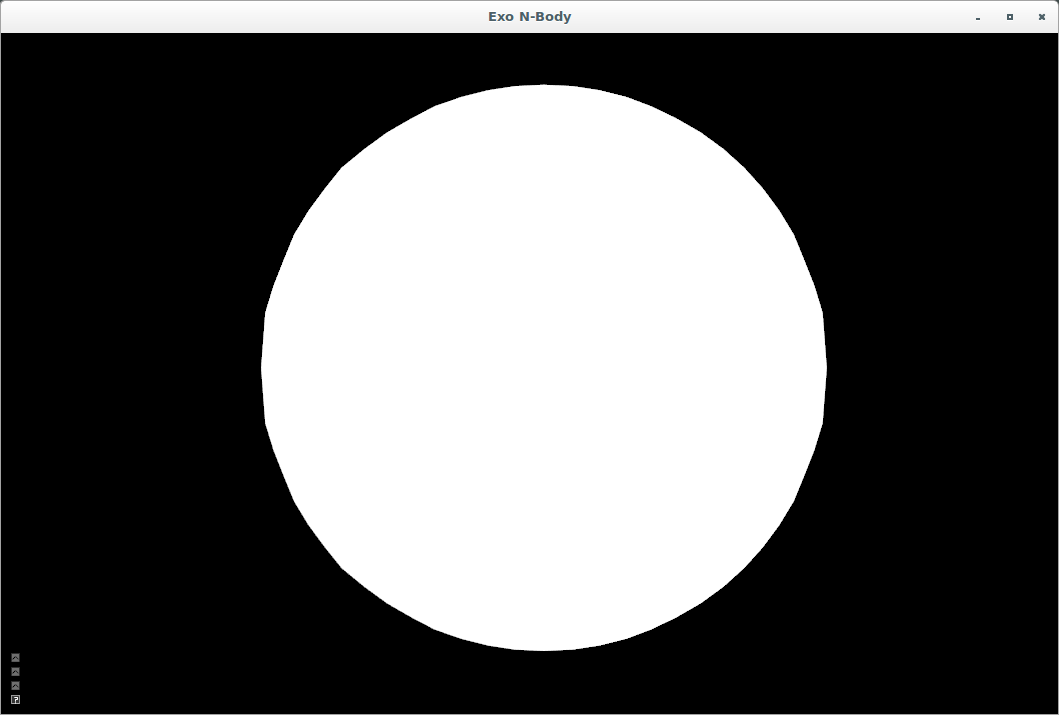
\includegraphics[width=0.9\textwidth]{img/testingEvidence/gui17_0.png}
  \caption{GUI17 - Body at 1E5.}
\end{figure}

\begin{figure}[H]
  \centering
  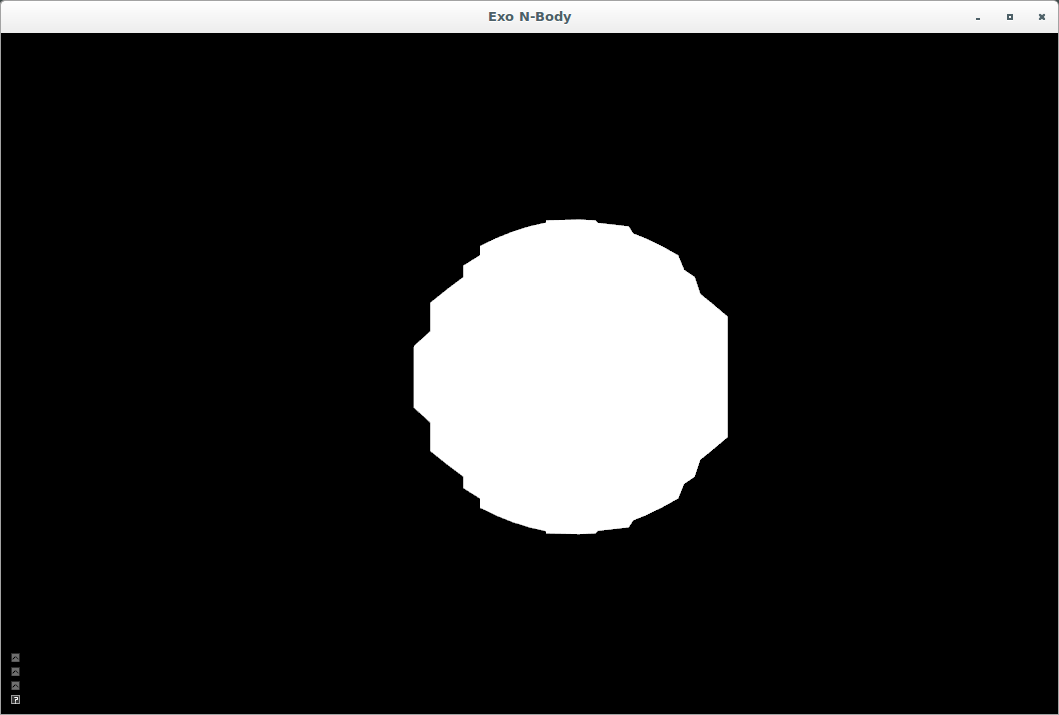
\includegraphics[width=0.9\textwidth]{img/testingEvidence/gui17_1.png}
  \caption{GUI17 - Body at 1E6.}
\end{figure}

\begin{figure}[H]
  \centering
  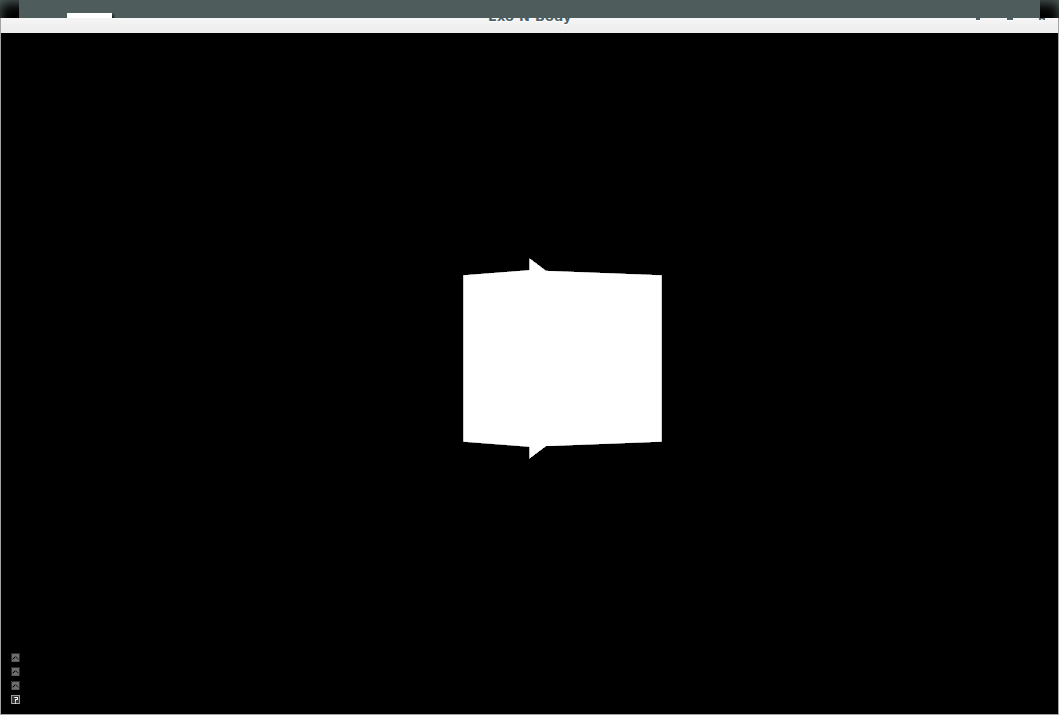
\includegraphics[width=0.9\textwidth]{img/testingEvidence/gui17_2.png}
  \caption{GUI17 - Body at 1E7.}
\end{figure}

\begin{figure}[H]
  \centering
  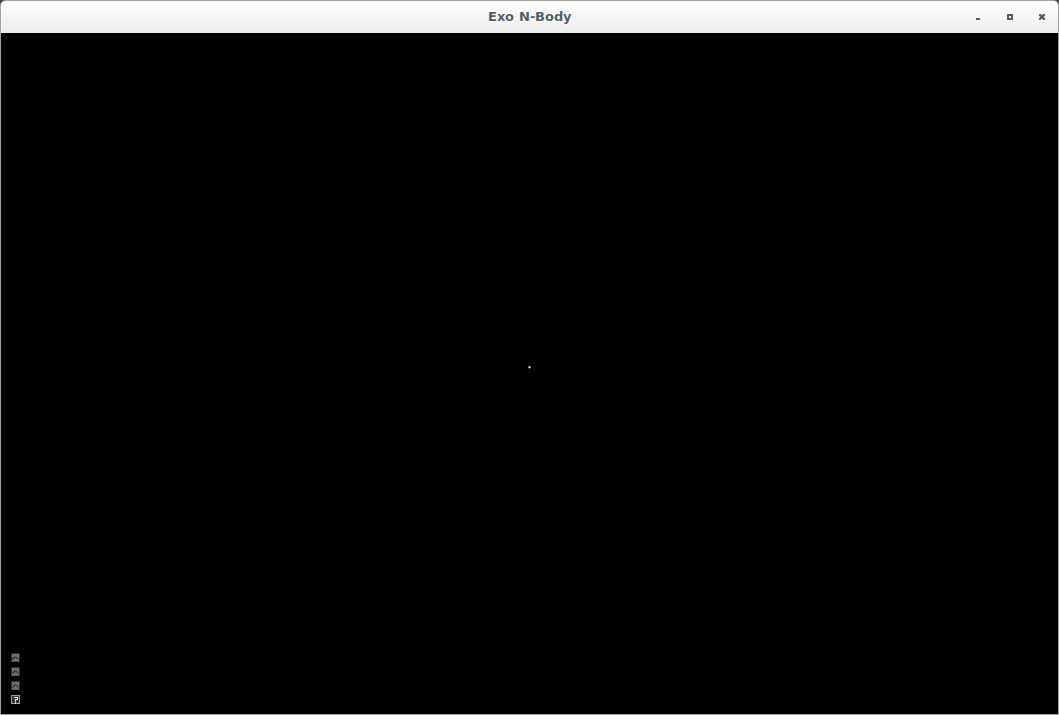
\includegraphics[width=0.9\textwidth]{img/testingEvidence/gui17_3.png}
  \caption{GUI17 - Body at 1E8.}
\end{figure}

\subsubsection{Simulation Tests}

\begin{figure}[H]
  \centering
  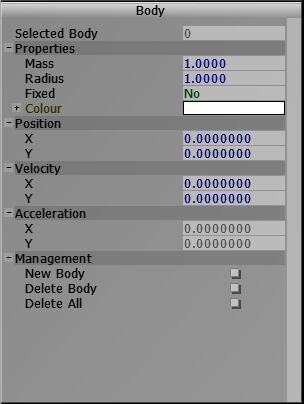
\includegraphics[width=0.4\textwidth]{img/testingEvidence/sim1.png}
  \caption{SIM1 - Body Remains Still.}
\end{figure}

\begin{figure}[H]
  \centering
  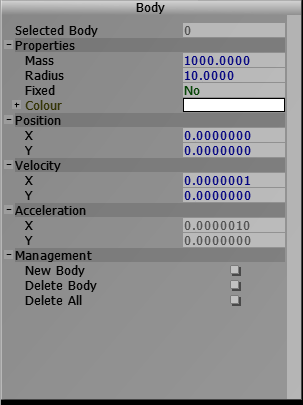
\includegraphics[width=0.4\textwidth]{img/testingEvidence/sim2.png}
  \caption{SIM2 - Acceleration on central body = 1E-6.}
\end{figure}

\begin{figure}[H]
  \centering
  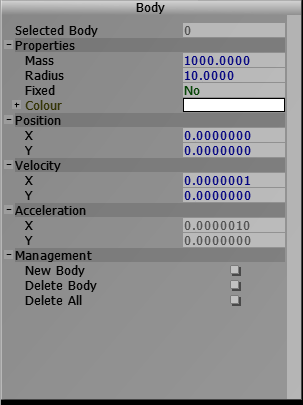
\includegraphics[width=0.4\textwidth]{img/testingEvidence/sim2.png}
  \caption{SIM3 - Acceleration on outer body = 1E-2.}
\end{figure}

\textbf{SIM5 Check:} \\
\textbf{0} - B0: [0.0128,0.0002] \hspace{20pt} B1: [87.1276,49.0818] \hspace{20pt} CD: [87.1148,49.0816] \\
    VD: $\sqrt{87.1148^2 + 49.0816^2} = 99.99$ \\

\textbf{1} - B0: [0.0197,0.0359] \hspace{20pt} B1: [-97.4692,-22.2332] \hspace{20pt} CD: [97.4889,22.2691] \\
    VD: $\sqrt{97.4889^2 + 22.2691^2} = 99.99$ \\
    
\textbf{SIM7 Check: (Mass)} \\
\textbf{0} - $1 + 1 = 2$ \hspace{10pt} \textbf{1} - $10 + 1 = 11$ \hspace{10pt} \textbf{2} - $20 + 100 = 120$ \hspace{10pt} \textbf{3} - $1000 + 1000 = 2000$ \\


\begin{wrapfigure}{hr}{0.5\textwidth}
  \centering
  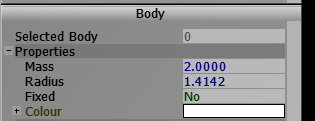
\includegraphics[width=0.4\textwidth]{img/testingEvidence/sim9.png}
  \caption{SIM7+9 - Radius and Mass}
\end{wrapfigure}

\textbf{SIM8 Check: (Velocity)} \\
$p=mv$ \hspace{20pt} $mv+mv=mv$ \\
\textbf{0} - 2 and -2, Final Velocity = 0.5 \\
\textbf{1} - 1 and -1, Final Velocity = 0.0 \\
\textbf{2} - 2 and  1, Final Velocity = 1.5 \\
\textbf{3} - -150 and 150, See Previous Notes. \\

\pagebreak

\begin{figure}[H]
  \centering
  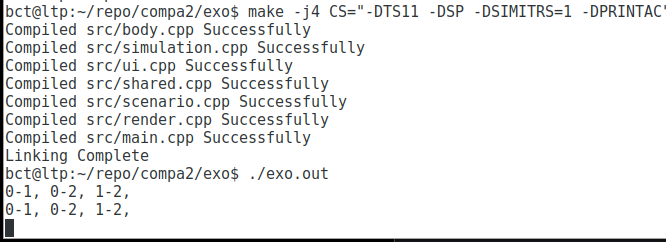
\includegraphics[width=\textwidth]{img/testingEvidence/sim18.png}
  \caption{SIM18 - Force calculation loop is correct.}
\end{figure}

\begin{figure}[H]
  \centering
  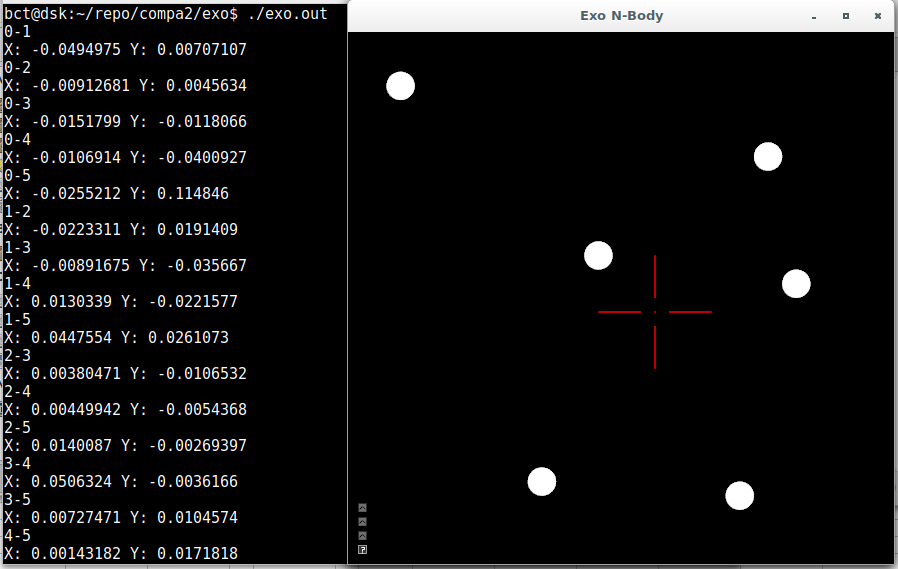
\includegraphics[width=\textwidth]{img/testingEvidence/sim19.png}
  \caption{SIM19 - All forces calculated correctly.}
\end{figure}

\pagebreak